% Options for packages loaded elsewhere
\PassOptionsToPackage{unicode}{hyperref}
\PassOptionsToPackage{hyphens}{url}
%
\documentclass[
]{book}
\usepackage{amsmath,amssymb}
\usepackage{iftex}
\ifPDFTeX
  \usepackage[T1]{fontenc}
  \usepackage[utf8]{inputenc}
  \usepackage{textcomp} % provide euro and other symbols
\else % if luatex or xetex
  \usepackage{unicode-math} % this also loads fontspec
  \defaultfontfeatures{Scale=MatchLowercase}
  \defaultfontfeatures[\rmfamily]{Ligatures=TeX,Scale=1}
\fi
\usepackage{lmodern}
\ifPDFTeX\else
  % xetex/luatex font selection
\fi
% Use upquote if available, for straight quotes in verbatim environments
\IfFileExists{upquote.sty}{\usepackage{upquote}}{}
\IfFileExists{microtype.sty}{% use microtype if available
  \usepackage[]{microtype}
  \UseMicrotypeSet[protrusion]{basicmath} % disable protrusion for tt fonts
}{}
\makeatletter
\@ifundefined{KOMAClassName}{% if non-KOMA class
  \IfFileExists{parskip.sty}{%
    \usepackage{parskip}
  }{% else
    \setlength{\parindent}{0pt}
    \setlength{\parskip}{6pt plus 2pt minus 1pt}}
}{% if KOMA class
  \KOMAoptions{parskip=half}}
\makeatother
\usepackage{xcolor}
\usepackage{color}
\usepackage{fancyvrb}
\newcommand{\VerbBar}{|}
\newcommand{\VERB}{\Verb[commandchars=\\\{\}]}
\DefineVerbatimEnvironment{Highlighting}{Verbatim}{commandchars=\\\{\}}
% Add ',fontsize=\small' for more characters per line
\usepackage{framed}
\definecolor{shadecolor}{RGB}{248,248,248}
\newenvironment{Shaded}{\begin{snugshade}}{\end{snugshade}}
\newcommand{\AlertTok}[1]{\textcolor[rgb]{0.94,0.16,0.16}{#1}}
\newcommand{\AnnotationTok}[1]{\textcolor[rgb]{0.56,0.35,0.01}{\textbf{\textit{#1}}}}
\newcommand{\AttributeTok}[1]{\textcolor[rgb]{0.13,0.29,0.53}{#1}}
\newcommand{\BaseNTok}[1]{\textcolor[rgb]{0.00,0.00,0.81}{#1}}
\newcommand{\BuiltInTok}[1]{#1}
\newcommand{\CharTok}[1]{\textcolor[rgb]{0.31,0.60,0.02}{#1}}
\newcommand{\CommentTok}[1]{\textcolor[rgb]{0.56,0.35,0.01}{\textit{#1}}}
\newcommand{\CommentVarTok}[1]{\textcolor[rgb]{0.56,0.35,0.01}{\textbf{\textit{#1}}}}
\newcommand{\ConstantTok}[1]{\textcolor[rgb]{0.56,0.35,0.01}{#1}}
\newcommand{\ControlFlowTok}[1]{\textcolor[rgb]{0.13,0.29,0.53}{\textbf{#1}}}
\newcommand{\DataTypeTok}[1]{\textcolor[rgb]{0.13,0.29,0.53}{#1}}
\newcommand{\DecValTok}[1]{\textcolor[rgb]{0.00,0.00,0.81}{#1}}
\newcommand{\DocumentationTok}[1]{\textcolor[rgb]{0.56,0.35,0.01}{\textbf{\textit{#1}}}}
\newcommand{\ErrorTok}[1]{\textcolor[rgb]{0.64,0.00,0.00}{\textbf{#1}}}
\newcommand{\ExtensionTok}[1]{#1}
\newcommand{\FloatTok}[1]{\textcolor[rgb]{0.00,0.00,0.81}{#1}}
\newcommand{\FunctionTok}[1]{\textcolor[rgb]{0.13,0.29,0.53}{\textbf{#1}}}
\newcommand{\ImportTok}[1]{#1}
\newcommand{\InformationTok}[1]{\textcolor[rgb]{0.56,0.35,0.01}{\textbf{\textit{#1}}}}
\newcommand{\KeywordTok}[1]{\textcolor[rgb]{0.13,0.29,0.53}{\textbf{#1}}}
\newcommand{\NormalTok}[1]{#1}
\newcommand{\OperatorTok}[1]{\textcolor[rgb]{0.81,0.36,0.00}{\textbf{#1}}}
\newcommand{\OtherTok}[1]{\textcolor[rgb]{0.56,0.35,0.01}{#1}}
\newcommand{\PreprocessorTok}[1]{\textcolor[rgb]{0.56,0.35,0.01}{\textit{#1}}}
\newcommand{\RegionMarkerTok}[1]{#1}
\newcommand{\SpecialCharTok}[1]{\textcolor[rgb]{0.81,0.36,0.00}{\textbf{#1}}}
\newcommand{\SpecialStringTok}[1]{\textcolor[rgb]{0.31,0.60,0.02}{#1}}
\newcommand{\StringTok}[1]{\textcolor[rgb]{0.31,0.60,0.02}{#1}}
\newcommand{\VariableTok}[1]{\textcolor[rgb]{0.00,0.00,0.00}{#1}}
\newcommand{\VerbatimStringTok}[1]{\textcolor[rgb]{0.31,0.60,0.02}{#1}}
\newcommand{\WarningTok}[1]{\textcolor[rgb]{0.56,0.35,0.01}{\textbf{\textit{#1}}}}
\usepackage{longtable,booktabs,array}
\usepackage{calc} % for calculating minipage widths
% Correct order of tables after \paragraph or \subparagraph
\usepackage{etoolbox}
\makeatletter
\patchcmd\longtable{\par}{\if@noskipsec\mbox{}\fi\par}{}{}
\makeatother
% Allow footnotes in longtable head/foot
\IfFileExists{footnotehyper.sty}{\usepackage{footnotehyper}}{\usepackage{footnote}}
\makesavenoteenv{longtable}
\usepackage{graphicx}
\makeatletter
\def\maxwidth{\ifdim\Gin@nat@width>\linewidth\linewidth\else\Gin@nat@width\fi}
\def\maxheight{\ifdim\Gin@nat@height>\textheight\textheight\else\Gin@nat@height\fi}
\makeatother
% Scale images if necessary, so that they will not overflow the page
% margins by default, and it is still possible to overwrite the defaults
% using explicit options in \includegraphics[width, height, ...]{}
\setkeys{Gin}{width=\maxwidth,height=\maxheight,keepaspectratio}
% Set default figure placement to htbp
\makeatletter
\def\fps@figure{htbp}
\makeatother
\setlength{\emergencystretch}{3em} % prevent overfull lines
\providecommand{\tightlist}{%
  \setlength{\itemsep}{0pt}\setlength{\parskip}{0pt}}
\setcounter{secnumdepth}{5}
\usepackage{booktabs}
\usepackage{lscape}

\ifLuaTeX
  \usepackage{selnolig}  % disable illegal ligatures
\fi
\usepackage[]{natbib}
\bibliographystyle{apalike}
\IfFileExists{bookmark.sty}{\usepackage{bookmark}}{\usepackage{hyperref}}
\IfFileExists{xurl.sty}{\usepackage{xurl}}{} % add URL line breaks if available
\urlstyle{same}
\hypersetup{
  pdftitle={Algoritma dan Pemrograman R},
  pdfauthor={Bakti Siregar, M.Sc},
  hidelinks,
  pdfcreator={LaTeX via pandoc}}

\title{Algoritma dan Pemrograman R}
\author{Bakti Siregar, M.Sc}
\date{20 Agustus 2022}

\begin{document}
\maketitle

{
\setcounter{tocdepth}{1}
\tableofcontents
}
\hypertarget{kata-pengantar}{%
\chapter*{Kata Pengantar}\label{kata-pengantar}}
\addcontentsline{toc}{chapter}{Kata Pengantar}

Bahasa pemrograman R telah menjadi alat yang kuat bagi para ilmuwan data, analis statistik, dan praktisi analisis numerik di seluruh dunia. Dengan kemampuan yang luar biasa dalam manipulasi data, visualisasi, dan analisis statistik, R memungkinkan para profesional untuk menggali wawasan berharga dari kumpulan data yang kompleks.

Dalam buku ini, penulis menyediakan materi dasar-dasar bahasa pemrograman R hingga tingkat yang lebih mendalam. Penulis juga menjelaskan beberapa konsep-konsep penting, sintaksis dasar, struktur data, serta memberikan contoh nyata tentang bagaimana R dapat digunakan dalam berbagai konteks. Modul ini dirancang untuk membantu pembaca yang baru mengenal pemrograman maupun yang telah memiliki pengalaman sebelumnya dalam bahasa lain.

\hypertarget{ringkasan-pembelajaran}{%
\section*{Ringkasan Pembelajaran}\label{ringkasan-pembelajaran}}
\addcontentsline{toc}{section}{Ringkasan Pembelajaran}

Adapun isi pembelajaran dalam modul ini adalah sebagai berikut:

\begin{itemize}
\tightlist
\item
  \textbf{Minggu 1-2: Dasar Pemrograman R}

  \begin{itemize}
  \tightlist
  \item
    Pengenalan konsep dasar pemrograman.
  \item
    Pengenalan lingkungan dan pengaturan awal bahasa R.
  \item
    Menulis program sederhana dalam R.
  \end{itemize}
\item
  \textbf{Minggu 3-4: Variabel dan Tipe Data}

  \begin{itemize}
  \tightlist
  \item
    Mengenal tipe data dasar dalam R: numerik, karakter, logika.
  \item
    Deklarasi dan penggunaan variabel.
  \item
    Konversi antar tipe data.
  \end{itemize}
\item
  \textbf{Minggu 5-6: Struktur Kontrol}

  \begin{itemize}
  \tightlist
  \item
    Penggunaan pernyataan kondisional (if, else).
  \item
    Penggunaan perulangan (for, while) untuk mengatur alur program.
  \item
    Studi kasus penggunaan struktur kontrol dalam pemrograman.
  \end{itemize}
\item
  \textbf{Minggu 7-8: Fungsi}

  \begin{itemize}
  \tightlist
  \item
    Pengenalan konsep fungsi dalam pemrograman.
  \item
    Membuat dan memanggil fungsi dalam R.
  \item
    Penggunaan parameter dalam fungsi.
  \end{itemize}
\item
  \textbf{Minggu 9-10: Struktur Data}

  \begin{itemize}
  \tightlist
  \item
    Pengenalan array dan matriks dalam R.
  \item
    Penggunaan vektor dan faktor.
  \item
    Pengenalan konsep dataframe untuk manipulasi data tabular.
  \end{itemize}
\item
  \textbf{Minggu 11-12: Algoritma Dasar}

  \begin{itemize}
  \tightlist
  \item
    Pengenalan konsep algoritma dan kompleksitas.
  \item
    Pemahaman tentang pencarian dan pengurutan.
  \item
    Implementasi algoritma pencarian dan pengurutan sederhana dalam R.
  \end{itemize}
\item
  \textbf{Minggu 13-14: Pengenalan Analisis Data}

  \begin{itemize}
  \tightlist
  \item
    Pengenalan pustaka dasar untuk analisis data di R.
  \item
    Pemahaman tentang statistik dasar dan visualisasi data.
  \item
    Penerapan analisis sederhana pada dataset kecil.
  \end{itemize}
\item
  \textbf{Minggu 15-16: Proyek Akhir}
  Siswa diminta untuk membuat proyek kecil menggunakan R yang menggabungkan konsep-konsep yang telah dipelajari. Proyek dapat berupa analisis data, pemecahan masalah, atau aplikasi sederhana.
\end{itemize}

\hypertarget{tim-penyusun}{%
\section*{Tim Penyusun}\label{tim-penyusun}}
\addcontentsline{toc}{section}{Tim Penyusun}

Berikut ini adalah nama dan biografi singkat para penulis:

\begin{itemize}
\tightlist
\item
  \textbf{Bakti Siregar, M.Sc} adalah Ketua Program Studi di Jurusan Statistika Universitas Matana. Lulusan Magister Matematika Terapan dari National Sun Yat Sen University, Taiwan. Beliau juga merupakan dosen dan konsultan Data Scientist di perusahaan-perusahaan ternama seperti \href{https://www.jne.co.id/id/beranda}{JNE}, \href{https://www.samoragroup.co.id/home/en}{Samora Group}, \href{https://www.pertamina.com/}{Pertamina}, dan lainnya. Beliau memiliki antusiasme khusus dalam mengajar Big Data Analytics, Machine Learning, Optimisasi, dan Analisis Time Series di bidang keuangan dan investasi. Keahliannya juga terlihat dalam penggunaan bahasa pemrograman Statistik seperti R Studio dan Python. Beliau mengaplikasikan sistem basis data MySQL/NoSQL dalam pembelajaran manajemen data, serta mahir dalam menggunakan tools Big Data seperti Spark dan Hadoop. Beberapa project beliau dapat dilihat di link berikut: \href{https://rpubs.com/dsciencelabs}{Rpubs}, \href{https://github.com/dsciencelabs}{Github}, \href{https://dsciencelabs.github.io/web/index.html}{Website}, dan \href{https://www.kaggle.com/baktisiregar/code}{Kaggle}.
\end{itemize}

\hypertarget{ucapan-terima-kasih}{%
\section*{Ucapan Terima Kasih}\label{ucapan-terima-kasih}}
\addcontentsline{toc}{section}{Ucapan Terima Kasih}

Kami berharap modul ini akan menjadi panduan yang bermanfaat bagi Anda dalam menguasai bahasa pemrograman R. Semoga dengan memahami konsep-konsep yang disajikan dalam modul ini, Anda akan dapat mengaplikasikan R dalam proyek-proyek analisis data dan statistik yang sebenarnya.

Terima kasih kepada semua yang telah berkontribusi dalam pembuatan modul ini, serta kepada Anda, pembaca, yang telah memilih modul ini sebagai sumber pengetahuan Anda. Kami berharap Anda menikmati perjalanan Anda dalam memahami bahasa pemrograman R.

\hypertarget{masukan-saran}{%
\section*{Masukan \& Saran}\label{masukan-saran}}
\addcontentsline{toc}{section}{Masukan \& Saran}

Semua masukan dan tanggapan Anda sangat berarti bagi kami untuk memperbaiki modul ini kedepannya. Bagi para pembaca/pengguna yang ingin menyampaikan masukan dan tanggapan, dipersilahkan melalui kontak dibawak ini!

\textbf{Email:} \href{mailto:dsciencelabs@outlook.com}{\nolinkurl{dsciencelabs@outlook.com}}

\hypertarget{pengenalan-r}{%
\chapter{Pengenalan R?}\label{pengenalan-r}}

R adalah bahasa pemrograman dan lingkungan komputasi yang digunakan untuk analisis statistik, visualisasi data, pengolahan data, dan pemodelan prediktif. R dikembangkan oleh Ross Ihaka dan Robert Gentleman di Universitas Auckland, Selandia Baru. R menjadi populer dalam dunia analisis data dan ilmu data karena kemampuannya dalam mengolah dan menganalisis data secara efisien.

\hypertarget{fitur-utama-r}{%
\section{Fitur Utama R}\label{fitur-utama-r}}

\begin{enumerate}
\def\labelenumi{\arabic{enumi}.}
\tightlist
\item
  \textbf{Open Source:} R adalah perangkat lunak open source yang dapat diunduh dan digunakan secara gratis.
\item
  \textbf{Fleksibilitas:} Anda dapat membuat fungsi sendiri, mengontrol alur program, dan mengakses berbagai pustaka eksternal.
\item
  \textbf{Mengimpor dan Mengekspor Data:} R mendukung berbagai format file, seperti CSV, Excel, SQL, dan format data lainnya.
\item
  \textbf{Data Manipulasi:} R memiliki pustaka seperti dplyr dan tidyr yang memudahkan manipulasi dan transformasi data.
\item
  \textbf{Lingkungan Komputasi:} R tidak hanya bahasa pemrograman, tetapi juga lingkungan komputasi lengkap yang menyediakan alat untuk analisis dan visualisasi data.
\item
  \textbf{Statistik dan Analisis Data:} R memiliki beragam pustaka dan paket yang mendukung analisis statistik, visualisasi data, dan pemodelan prediktif.
\item
  \textbf{Grafik dan Visualisasi:} R memiliki kemampuan visualisasi yang kuat dengan pustaka seperti ggplot2 untuk membuat grafik yang informatif dan menarik.
\item
  \textbf{Komunitas Aktif:} Komunitas R sangat aktif, dan ada banyak sumber daya online, forum, dan pustaka yang dapat membantu dalam pembelajaran dan pemecahan masalah.
\end{enumerate}

\hypertarget{mengapa-belajar-r}{%
\section{Mengapa Belajar R?}\label{mengapa-belajar-r}}

Berikut ini adalah beberapa alasan mengapa penting untuk belajar R:

\begin{enumerate}
\def\labelenumi{\arabic{enumi}.}
\tightlist
\item
  \textbf{Pengolahan Data:} R dapat membantu Anda membersihkan, merubah format, dan mengolah data sebelum analisis lebih lanjut.
\item
  \textbf{Analisis Data:} R adalah alat yang kuat untuk menganalisis data, membuat visualisasi yang menarik, dan mengidentifikasi pola dalam dataset.
\item
  \textbf{Karir di Ilmu Data:} Penguasaan R menjadi salah satu keahlian yang sangat dihargai dalam industri ilmu data dan analisis data.
\item
  \textbf{Komunitas Besar:} Anda akan menjadi bagian dari komunitas besar yang mendukung dan berkontribusi dalam pengembangan R serta membagikan pengetahuan.
\end{enumerate}

\hypertarget{download-r-rstudio}{%
\section{Download R \& Rstudio:}\label{download-r-rstudio}}

\begin{enumerate}
\def\labelenumi{\arabic{enumi}.}
\tightlist
\item
  \textbf{Unduh dan Instalasi:} Kunjungi situs resmi R (\url{https://www.r-project.org/}) untuk mengunduh installer sesuai dengan sistem operasi Anda.
\item
  \textbf{RStudio (Opsional tapi Disarankan):} RStudio adalah lingkungan pengembangan terintegrasi (IDE) yang mempermudah pengembangan dalam R. Anda dapat mengunduh RStudio (\url{https://www.rstudio.com/}) dan menggunakannya untuk menulis dan menjalankan kode R.
\end{enumerate}

\hypertarget{tutorial-instal-r-studio}{%
\section{Tutorial Instal R \& Studio}\label{tutorial-instal-r-studio}}

Berikut adalah panduan langkah demi langkah untuk menginstal R dan RStudio

\hypertarget{instalasi-r}{%
\subsection{Instalasi R}\label{instalasi-r}}

R adalah bahasa pemrograman inti yang digunakan oleh RStudio. Ikuti langkah-langkah di bawah ini untuk menginstal R:

\hypertarget{windows}{%
\subsubsection*{Windows}\label{windows}}
\addcontentsline{toc}{subsubsection}{Windows}

\begin{enumerate}
\def\labelenumi{\arabic{enumi}.}
\tightlist
\item
  Kunjungi situs resmi R di \url{https://cran.r-project.org/mirrors.html}.
\item
  Pilih cermin (mirror) terdekat untuk mengunduh installer R.
\item
  Unduh installer R untuk Windows dan jalankan file installer yang diunduh.
\item
  Ikuti panduan instalasi, pilih opsi default kecuali jika Anda tahu persis apa yang Anda lakukan.
\item
  Setelah instalasi selesai, R akan terinstal di komputer Anda.
\end{enumerate}

\hypertarget{macos}{%
\subsubsection*{MacOS}\label{macos}}
\addcontentsline{toc}{subsubsection}{MacOS}

\begin{enumerate}
\def\labelenumi{\arabic{enumi}.}
\tightlist
\item
  Kunjungi situs resmi R di \url{https://cran.r-project.org/mirrors.html}.
\item
  Pilih cermin (mirror) terdekat untuk mengunduh installer R.
\item
  Unduh installer R untuk macOS dan jalankan file installer yang diunduh.
\item
  Ikuti panduan instalasi, pilih opsi default kecuali jika Anda tahu persis apa yang Anda lakukan.
\item
  Setelah instalasi selesai, R akan terinstal di komputer Anda.
\end{enumerate}

\hypertarget{linux}{%
\subsubsection*{Linux}\label{linux}}
\addcontentsline{toc}{subsubsection}{Linux}

Di sistem Linux, Anda dapat menggunakan perintah terminal untuk menginstal R. Berikut adalah contoh untuk beberapa distribusi umum:

\textbf{Ubuntu/Debian:}

Buka Program \texttt{csharp} anda dan run koding dibawah ini!

\begin{verbatim}
Copy code
sudo apt-get update
sudo apt-get install r-base
\end{verbatim}

\textbf{CentOS/Fedora:}

Buka Program \texttt{Command\ Prompt} anda dan run koding dibawah ini!

\begin{verbatim}
sudo yum install R
\end{verbatim}

\hypertarget{instalasi-rstudio}{%
\subsection{Instalasi RStudio:}\label{instalasi-rstudio}}

RStudio adalah Integrated Development Environment (IDE) yang mempermudah pengembangan dalam R. Ikuti langkah-langkah di bawah ini untuk menginstal RStudio:

\textbf{Windows, macOS, dan Linux:}

\begin{enumerate}
\def\labelenumi{\arabic{enumi}.}
\tightlist
\item
  Kunjungi situs resmi RStudio di \url{https://www.rstudio.com/products/rstudio/download/}.
\item
  Pilih ``RStudio Desktop'' yang sesuai dengan sistem operasi Anda.
\item
  Unduh installer RStudio dan jalankan file installer yang diunduh.
\item
  Ikuti panduan instalasi dan pilih opsi default kecuali jika Anda tahu persis apa yang Anda lakukan.
\item
  Setelah instalasi selesai, RStudio akan terinstal di komputer Anda.
\end{enumerate}

\hypertarget{video-instalasi-r-rstudio}{%
\section{Video Instalasi R \& RStudio}\label{video-instalasi-r-rstudio}}

\hypertarget{windows-1}{%
\subsection{Windows}\label{windows-1}}

\hypertarget{macos-1}{%
\subsection{MacOS}\label{macos-1}}

\hypertarget{interface-r-rstudio}{%
\section{Interface R \& RStudio:}\label{interface-r-rstudio}}

Interface adalah tampilan aplikasi R dan Rstudio yang telah terpasang diperlihatkan pada Gambar \ref{fig:jendela-R} dan Gambar \ref{fig:jendela-RStudio}.

\begin{figure}

{\centering 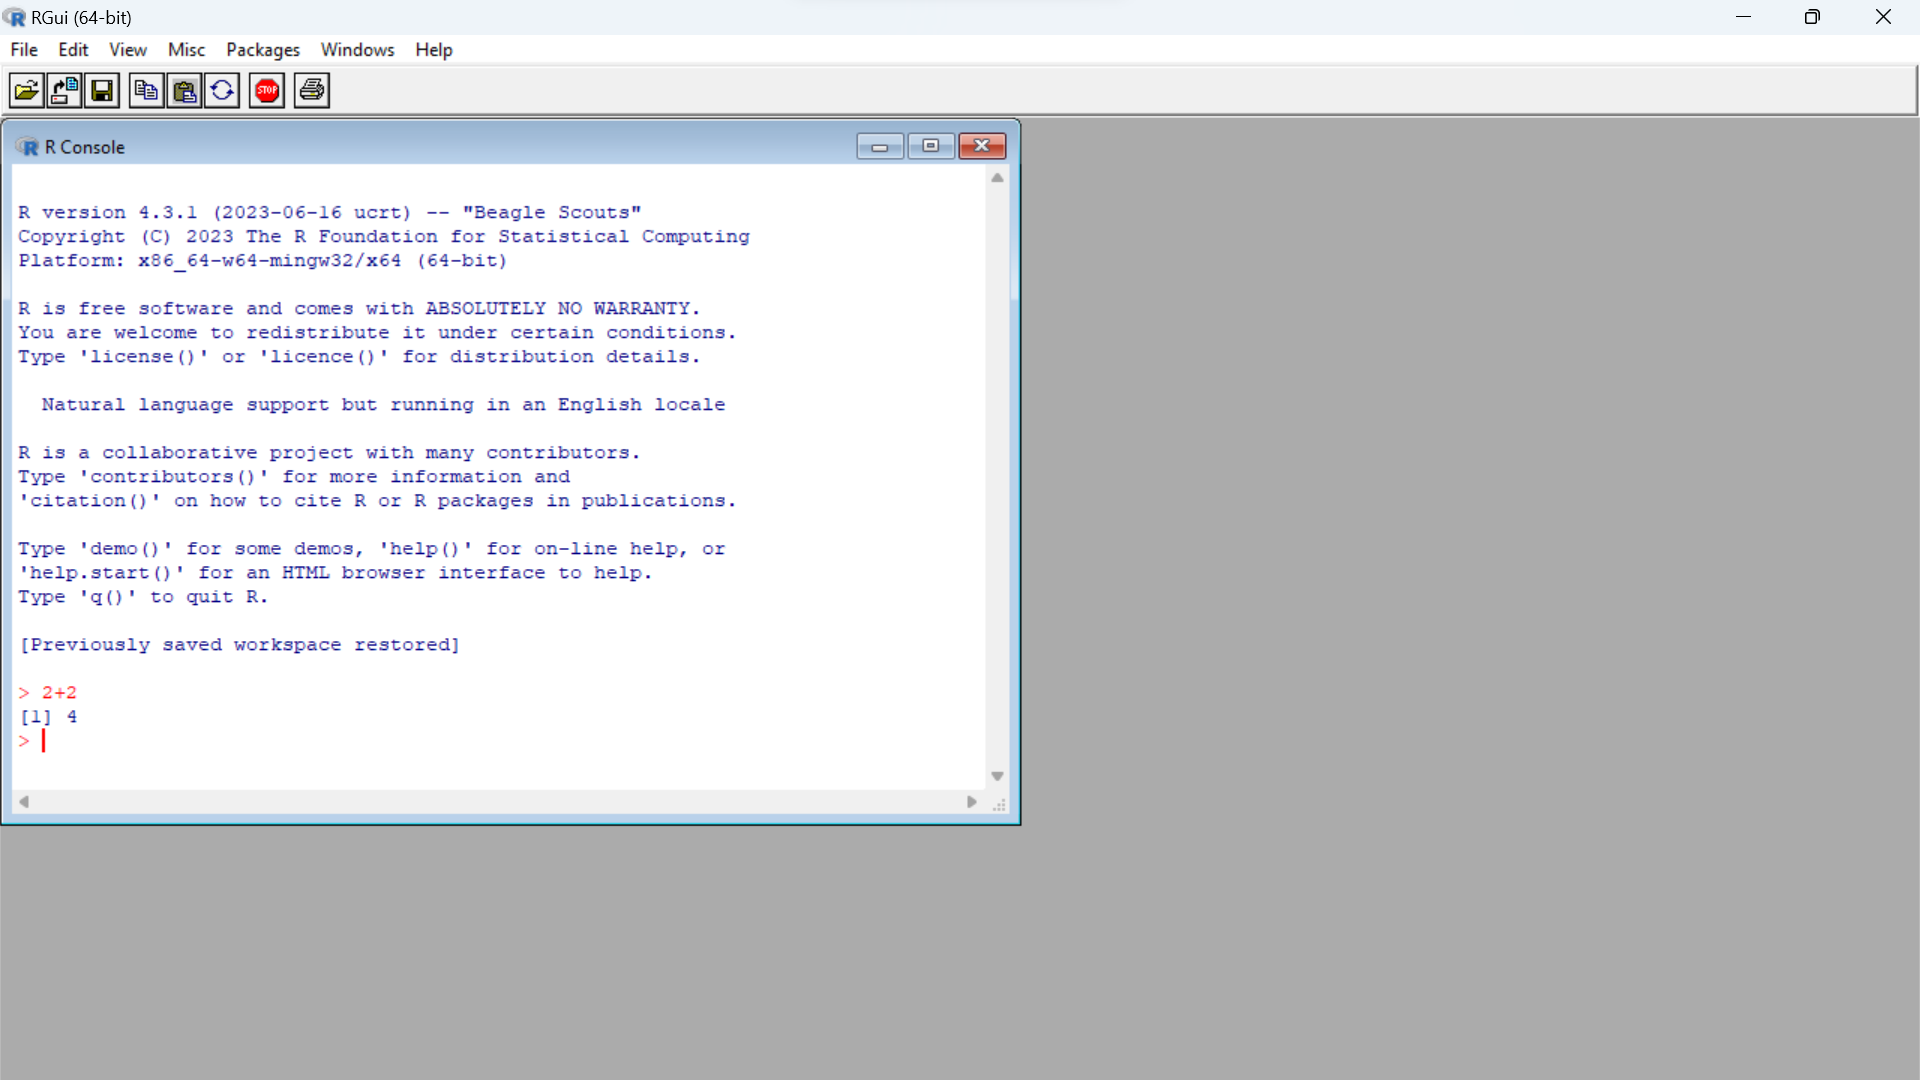
\includegraphics[width=1\linewidth]{./images/Bab1/jendela_r} 

}

\caption{Jendela R.}\label{fig:jendela-R}
\end{figure}

\begin{figure}

{\centering 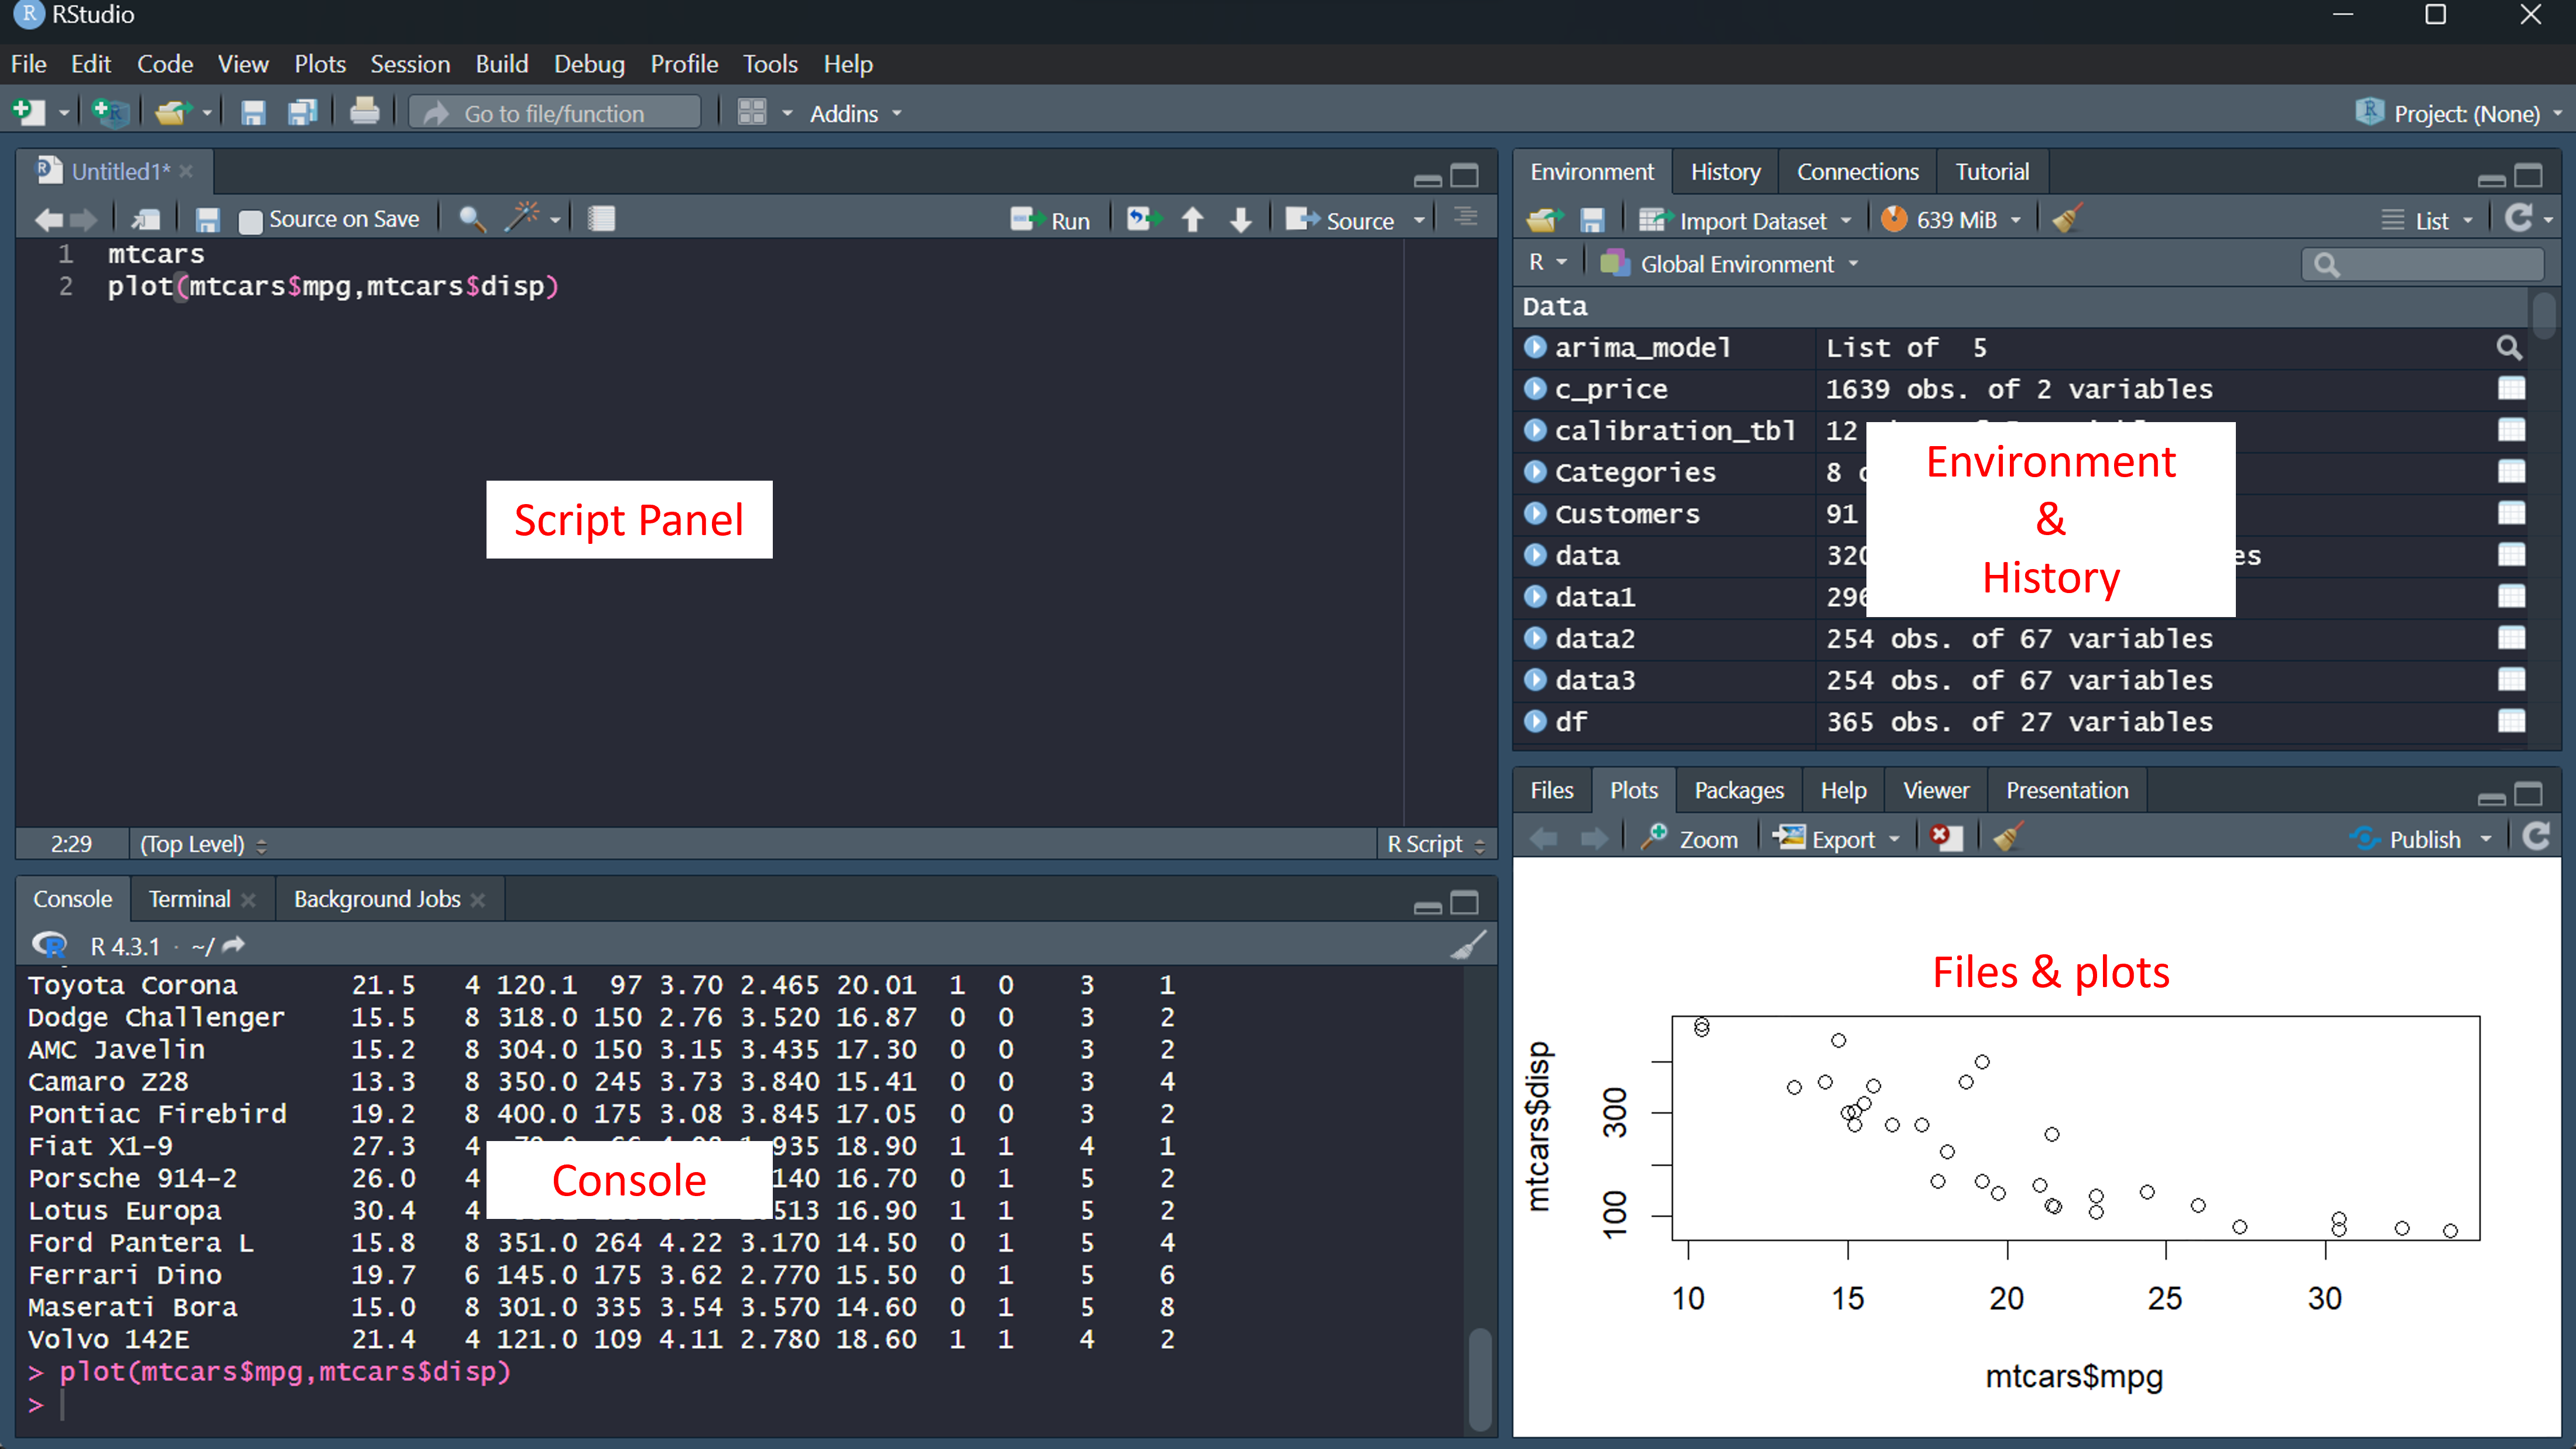
\includegraphics[width=1\linewidth]{./images/Bab1/Rstudio} 

}

\caption{Jendela RStudio.}\label{fig:jendela-RStudio}
\end{figure}

Tampilan ini memiliki beberapa komponen utama, termasuk:

\begin{itemize}
\tightlist
\item
  \textbf{Script Panel:} Tempat Anda menulis kode R dalam skrip.
\item
  \textbf{Console Panel:} Tempat hasil dari kode R ditampilkan, serta tempat Anda dapat menjalankan kode secara interaktif.
\item
  \textbf{Environment Panel:} Menampilkan daftar variabel yang ada dalam sesi R Anda.
\item
  \textbf{History Panel:} Menampilkan riwayat perintah yang telah dijalankan.
\item
  \textbf{Files/Plots/Packages/Help Panel:} Panel tambahan yang membantu Anda mengelola file, visualisasi, pustaka, dan panduan bantuan.
\end{itemize}

Interface ini memudahkan pengguna untuk menulis, menjalankan, dan mengelola kode R serta menganalisis data dengan nyaman.

\hypertarget{sintaks-dasar-r}{%
\section{Sintaks Dasar R}\label{sintaks-dasar-r}}

Berikut ini beberapa kode sederhana yang bisa dipelajari untuk memulai memahami cara kerja Bahasa pemrograman R.

\begin{verbatim}
3+7
3-7
3^7
3/7
3*7
9^(1/3)
\end{verbatim}

\hypertarget{bantuan-help-r}{%
\section{Bantuan (Help) R}\label{bantuan-help-r}}

Salah satu bagian terpenting dalam bekerja dengan bahasa R adalah mengetahui di mana mencari bantuan. R memiliki beberapa fasilitas in-line, selain berbagai sumber daya bantuan di ekosistem R. Anda dapat menggunakan bantuan untuk fungsi tertentu.

\begin{Shaded}
\begin{Highlighting}[]
\FunctionTok{help.start}\NormalTok{()         }\CommentTok{\# menu di mana Anda dapat menavigasi bantuan lokal berbasis web}
\NormalTok{?help                }\CommentTok{\# menu di mana Anda dapat menavigasi bantuan lokal berbasis web }
\NormalTok{?class               }\CommentTok{\# mendapatkan bantuan untuk fungsi \textasciigrave{}class\textasciigrave{}}
\FunctionTok{help}\NormalTok{(class)          }\CommentTok{\# mendapatkan bantuan untuk fungsi \textasciigrave{}class\textasciigrave{}}
\NormalTok{??class              }\CommentTok{\# jika Anda tidak tahu nama fungsi yang Anda cari}
\FunctionTok{help.search}\NormalTok{(}\StringTok{\textquotesingle{}class\textquotesingle{}}\NormalTok{) }\CommentTok{\# jika Anda tidak tahu nama fungsi yang Anda cari}
\end{Highlighting}
\end{Shaded}

\hypertarget{shortcut-penggunaan-rstudio}{%
\section{Shortcut Penggunaan Rstudio}\label{shortcut-penggunaan-rstudio}}

Beberapa petunjuk bermanfaat untuk Rstudio (IDE) meliputi:

\begin{longtable}[]{@{}lcc@{}}
\toprule\noalign{}
Kata Kunci & Perintah & Detail \\
\midrule\noalign{}
\endhead
\bottomrule\noalign{}
\endlastfoot
Ctrl + Return (Enter) & untuk menjalankan baris dari editor & \textasciitilde{} \\
Ctrl + Shift + \# & untuk fokus pada tab bantuan & kontradiktif \\
Alt + Shift + k & untuk jalur pintas keyboard RStudio & \textasciitilde{} \\
Ctrl + r & untuk menelusuri sejarah perintah & \textasciitilde{} \\
Alt + Shift + j & untuk menavigasi antar bagian kode & \textasciitilde{} \\
Ctrl + 1 & untuk melompat ke editor & tab untuk penyelesaian otomatis \\
Ctrl + 2 & untuk melompat ke konsol & tab untuk penyelesaian otomatis \\
Ctrl + 8 & untuk melompat ke environment list & tab untuk pelengkapan otomatis \\
Alt + l & Collapse chunk & Code Folding \\
Alt + Shift + l & Unfold chunk & Code Folding \\
Alt + o & Collapse all & Code Folding \\
Alt + Shift + o & Unfold all & Code Folding \\
Alt + ``-'' & untuk operator penugasan \textless- & \textasciitilde{} \\
Alt + Shift + c & kode komentar/tanda komentar dalam file & .R kontradiktif \\
\end{longtable}

\hypertarget{praktikum}{%
\section{Praktikum}\label{praktikum}}

Buatlah tutorial Instalasi R dan R Studio dalam M.word! Lengkapi setiap prosesnya dengan gambar dan penjelasan.

\hypertarget{dasar-pemrograman-r}{%
\chapter{Dasar Pemrograman R}\label{dasar-pemrograman-r}}

Pemrograman R merujuk pada proses menulis kode dan mengembangkan program menggunakan bahasa pemrograman R. R adalah bahasa pemrograman yang fokus pada analisis statistik, manipulasi data, dan visualisasi. Pada bab ini akan dibahas beberapa unsur utama dalam pemrograman menggunakan bahasa pemrograman R.

\hypertarget{variabel}{%
\section{Variabel}\label{variabel}}

Variabel dalam bahasa pemrograman R digunakan untuk menyimpan dan mengelola data. Variabel memungkinkan Anda untuk menampung nilai-nilai berbagai jenis, seperti angka, karakter (teks), atau nilai logika (benar/salah). Berikut ini adalah cara untuk mendefinisikan dan menggunakan variabel dalam R:

\hypertarget{mendefinisikan-variabel}{%
\subsection{Mendefinisikan Variabel}\label{mendefinisikan-variabel}}

Untuk membuat variabel, Anda cukup menggunakan tanda \textless- atau = untuk memberikan nilai pada variabel.

\begin{Shaded}
\begin{Highlighting}[]
\NormalTok{x }\OtherTok{\textless{}{-}} \DecValTok{10}          \CommentTok{\# Mendefinisikan variabel x }
\NormalTok{y }\OtherTok{=} \DecValTok{12}           \CommentTok{\# Mendefinisikan variabel y}
\end{Highlighting}
\end{Shaded}

\hypertarget{aturan-nama-variabel}{%
\subsection{Aturan Nama Variabel}\label{aturan-nama-variabel}}

\begin{itemize}
\tightlist
\item
  Nama variabel harus dimulai dengan huruf atau tanda \texttt{.}
\item
  Nama variabel bisa terdiri dari huruf, angka, dan tanda \texttt{\_}.
\item
  Karakter khusus seperti +, -, *, /, \^{} dll. tidak diperbolehkan dalam nama variabel.
\item
  Nama variabel bersifat case-sensitive, artinya \texttt{x} dan \texttt{X} dianggap berbeda.
\end{itemize}

\hypertarget{operator}{%
\section{Operator}\label{operator}}

Operator adalah simbol yang mengarahkan compiler untuk melakukan berbagai macam operasi terhadap beberapa penugasan. Operator mensimulasikan berbagai operasi matematis, logika, dan keputusan yang dilakukan pada sekumpulan Bilangan Kompleks, Integer, dan Numerik sebagai penugasan masukan (input). R mendukung sebagian besar empat jenis operator biner antara satu set penugasan. Dalam ini, kita akan melihat berbagai jenis operator yang tersedia di R penggunaannya.

\hypertarget{aritmatika}{%
\subsection{Aritmatika}\label{aritmatika}}

Penggunaan operator aritmatika dalam program R adalah untuk mensimulasikan berbagai operasi matematika, seperti penambahan, pengurangan, perkalian, pembagian, dan modulo. Operator aritmatika yang dilakukan bisa saja berupa nilai skalar, bilangan kompleks, atau vektor.

\begin{longtable}[]{@{}cc@{}}
\toprule\noalign{}
\endhead
\bottomrule\noalign{}
\endlastfoot
\textbf{Operator} & \textbf{R} \\
Penjumlahan & + \\
Pengurangan & - \\
Perkalian & * \\
Divisi/Pembagian & / \\
Pemangkatan & \^{} \\
Modulo & \%\% \\
\end{longtable}

Perhatikan cuplikan R berikut:

\begin{Shaded}
\begin{Highlighting}[]
\NormalTok{x }\OtherTok{\textless{}{-}} \FunctionTok{c}\NormalTok{(}\DecValTok{2}\NormalTok{,}\DecValTok{3}\NormalTok{,}\DecValTok{5}\NormalTok{)    }\CommentTok{\# memuat vektor x}
\NormalTok{y }\OtherTok{\textless{}{-}} \FunctionTok{c}\NormalTok{(}\DecValTok{2}\NormalTok{,}\DecValTok{4}\NormalTok{,}\DecValTok{6}\NormalTok{)    }\CommentTok{\# memuat vektor y}
\NormalTok{x}\SpecialCharTok{+}\NormalTok{y              }\CommentTok{\# hasil penjumahan vektor x dan y}
\FunctionTok{print}\NormalTok{ (x}\SpecialCharTok{+}\NormalTok{y)      }\CommentTok{\# hasil penjumahan vektor x dan y}
\FunctionTok{print}\NormalTok{ (x}\SpecialCharTok{{-}}\NormalTok{y)      }\CommentTok{\# hasil pengurangan vektor x dan y}
\FunctionTok{print}\NormalTok{ (x}\SpecialCharTok{*}\NormalTok{y)      }\CommentTok{\# hasil perkalian vektor x dan y}
\FunctionTok{print}\NormalTok{ (x}\SpecialCharTok{/}\NormalTok{y)      }\CommentTok{\# hasil pembagian vektor x dan y}
\FunctionTok{print}\NormalTok{ (x}\SpecialCharTok{\^{}}\NormalTok{y)      }\CommentTok{\# hasil pemangkatan vektor x dan y}
\FunctionTok{print}\NormalTok{ (x}\SpecialCharTok{\%\%}\NormalTok{y)     }\CommentTok{\# hasil modulo vektor x dan y}
\end{Highlighting}
\end{Shaded}

Adakalanya anda perlu menampilkan keterangan/komentar yang juga melekat pada hasil perhitungan R itu sendiri. Maka anda dapat melakukannya dengan cara berikut:

\begin{Shaded}
\begin{Highlighting}[]
\FunctionTok{cat}\NormalTok{(}\StringTok{"Penjumahan vektor x dan y :"}\NormalTok{, x }\SpecialCharTok{+}\NormalTok{ y, }\StringTok{"}\SpecialCharTok{\textbackslash{}n}\StringTok{"}\NormalTok{)}
\FunctionTok{cat}\NormalTok{(}\StringTok{"Pengurangan vektor x dan y :"}\NormalTok{, x }\SpecialCharTok{{-}}\NormalTok{ y, }\StringTok{"}\SpecialCharTok{\textbackslash{}n}\StringTok{"}\NormalTok{)}
\FunctionTok{cat}\NormalTok{(}\StringTok{"Perkalian vektor x dan y :"}\NormalTok{, x }\SpecialCharTok{*}\NormalTok{ y, }\StringTok{"}\SpecialCharTok{\textbackslash{}n}\StringTok{"}\NormalTok{)}
\FunctionTok{cat}\NormalTok{(}\StringTok{"Pembagian vektor x dan y :"}\NormalTok{, x }\SpecialCharTok{/}\NormalTok{ y, }\StringTok{"}\SpecialCharTok{\textbackslash{}n}\StringTok{"}\NormalTok{)}
\FunctionTok{cat}\NormalTok{ (}\StringTok{"Pemangkatan vektor x dan y :"}\NormalTok{, x }\SpecialCharTok{\^{}}\NormalTok{ y) }
\FunctionTok{cat}\NormalTok{(}\StringTok{"Modulo vektor x dan y :"}\NormalTok{, x }\SpecialCharTok{\%\%}\NormalTok{ y, }\StringTok{"}\SpecialCharTok{\textbackslash{}n}\StringTok{"}\NormalTok{)}
\end{Highlighting}
\end{Shaded}

\textbf{Catatan:} Penjelasan lebih lekap mengenai modulo dapat lihat pada \href{https://www.omnicalculator.com/math/modulo}{link ini}

\hypertarget{relasional}{%
\subsection{Relasional}\label{relasional}}

Operator relasional melakukan operasi perbandingan antara elemen yang bersesuaian pada setiap operan. Mengembalikan nilai Boolean TRUE jika operan pertama memenuhi relasi dibandingkan dengan operan kedua. Nilai TRUE selalu dianggap lebih besar dari FALSE.

\begin{longtable}[]{@{}
  >{\centering\arraybackslash}p{(\columnwidth - 4\tabcolsep) * \real{0.3077}}
  >{\centering\arraybackslash}p{(\columnwidth - 4\tabcolsep) * \real{0.3077}}
  >{\centering\arraybackslash}p{(\columnwidth - 4\tabcolsep) * \real{0.3846}}@{}}
\toprule\noalign{}
\endhead
\bottomrule\noalign{}
\endlastfoot
\textbf{Operator} & \textbf{R} & \textbf{Keterangan} \\
Kurang dari & \textless{} & Mengembalikan TRUE jika elemen yang bersesuaian pada operan pertama lebih kecil dari operan kedua. Selain itu akan mengembalikan FALSE \\
Kurang dari sama dengan & \textless= & Mengembalikan TRUE jika elemen yang bersesuaian pada operan pertama kurang dari atau sama dengan elemen operan kedua. Selain itu akan mengembalikan FALSE \\
Lebih besar dari & \textgreater{} & Mengembalikan TRUE jika elemen yang bersesuaian pada operan pertama lebih besar dari operan kedua. Selain itu akan mengembalikan FALSE \\
Lebih besar dari sama dengan & \textgreater= & Mengembalikan BENAR jika elemen yang bersesuaian pada operan pertama lebih besar atau sama dengan dari operan kedua. Selain itu akan mengembalikan FALSE \\
Sama Dengan & == & Mengembalikan BENAR jika dan hanya jika kedua sisi bernilai sama \\
Tidak Sama dengan & != & Mengembalikan BENAR jika elemen yang bersesuaian pada operan pertama tidak sama dengan dari operan kedua \\
\end{longtable}

\begin{Shaded}
\begin{Highlighting}[]
\NormalTok{x }\OtherTok{\textless{}{-}} \FunctionTok{c}\NormalTok{(}\DecValTok{2}\NormalTok{,}\DecValTok{3}\NormalTok{,}\DecValTok{5}\NormalTok{)    }\CommentTok{\# memuat vektor x}
\NormalTok{y }\OtherTok{\textless{}{-}} \FunctionTok{c}\NormalTok{(}\DecValTok{2}\NormalTok{,}\DecValTok{4}\NormalTok{,}\DecValTok{6}\NormalTok{)    }\CommentTok{\# memuat vektor y}
\FunctionTok{cat}\NormalTok{(}\StringTok{"Vektor x  kurang dari Vektor y:"}\NormalTok{, x }\SpecialCharTok{\textless{}}\NormalTok{ y, }\StringTok{"}\SpecialCharTok{\textbackslash{}n}\StringTok{"}\NormalTok{)}
\FunctionTok{cat}\NormalTok{(}\StringTok{"Vector x kurang dari sama dengan Vector y:"}\NormalTok{, x }\SpecialCharTok{\textless{}=}\NormalTok{ y, }\StringTok{"}\SpecialCharTok{\textbackslash{}n}\StringTok{"}\NormalTok{)}
\FunctionTok{cat}\NormalTok{(}\StringTok{"Vector x lebih besar dari Vector y :"}\NormalTok{, x }\SpecialCharTok{\textgreater{}}\NormalTok{ y, }\StringTok{"}\SpecialCharTok{\textbackslash{}n}\StringTok{"}\NormalTok{)}
\FunctionTok{cat}\NormalTok{(}\StringTok{"Vector x lebih besar dari sama dengan Vector y :"}\NormalTok{, x }\SpecialCharTok{\textgreater{}=}\NormalTok{ y, }\StringTok{"}\SpecialCharTok{\textbackslash{}n}\StringTok{"}\NormalTok{)}
\FunctionTok{cat}\NormalTok{(}\StringTok{"Vector x sama dengan Vector y:"}\NormalTok{, x }\SpecialCharTok{==}\NormalTok{ y,}\StringTok{"}\SpecialCharTok{\textbackslash{}n}\StringTok{"}\NormalTok{) }
\FunctionTok{cat}\NormalTok{(}\StringTok{"Vector x tidak sama dengan Vector y:"}\NormalTok{, x }\SpecialCharTok{!=}\NormalTok{ y) }
\end{Highlighting}
\end{Shaded}

\hypertarget{logika}{%
\subsection{Logika}\label{logika}}

Operator logis mensimulasikan operasi keputusan, berdasarkan operator yang ditentukan antara operan, yang kemudian dievaluasi ke nilai Boolean Benar atau Salah. Nilai bilangan bulat bukan nol dianggap sebagai nilai BENAR, baik itu bilangan kompleks atau bilangan real.

\begin{longtable}[]{@{}
  >{\centering\arraybackslash}p{(\columnwidth - 4\tabcolsep) * \real{0.3077}}
  >{\centering\arraybackslash}p{(\columnwidth - 4\tabcolsep) * \real{0.3077}}
  >{\centering\arraybackslash}p{(\columnwidth - 4\tabcolsep) * \real{0.3846}}@{}}
\toprule\noalign{}
\endhead
\bottomrule\noalign{}
\endlastfoot
\textbf{Operator} & \textbf{R} & \textbf{Keterangan} \\
NOT & ! & Operasi negasi/kebalikan pada status elemen operan \\
AND & \& & Mengembalikan TRUE jika kedua operan bernilai Benar \\
OR & \(|\) & Mengembalikan TRUE jika salah satu operan adalah Benar \\
XOR & \^{} & Mengembalikan TRUE jika salah satu dari kedua elemen pertama operan bernilai Benar \\
\end{longtable}

\begin{Shaded}
\begin{Highlighting}[]
\NormalTok{x }\OtherTok{\textless{}{-}} \FunctionTok{c}\NormalTok{(}\DecValTok{0}\NormalTok{,}\ConstantTok{TRUE}\NormalTok{,}\ConstantTok{FALSE}\NormalTok{)}
\NormalTok{y }\OtherTok{\textless{}{-}} \FunctionTok{c}\NormalTok{(}\ConstantTok{TRUE}\NormalTok{,}\FloatTok{0.1}\NormalTok{,}\DecValTok{4}\SpecialCharTok{+}\NormalTok{3i)}
 
\CommentTok{\# Melakukan operasi logika pada Operan}
\FunctionTok{cat}\NormalTok{(}\StringTok{"Logika Negasi (\textasciitilde{}) untuk vektor x:"}\NormalTok{, }\SpecialCharTok{!}\NormalTok{x, }\StringTok{"}\SpecialCharTok{\textbackslash{}n}\StringTok{"}\NormalTok{) }
\FunctionTok{cat}\NormalTok{(}\StringTok{"Logika Negasi (\textasciitilde{}) untuk vektor y :"}\NormalTok{, }\SpecialCharTok{!}\NormalTok{y, }\StringTok{"}\SpecialCharTok{\textbackslash{}n}\StringTok{"}\NormalTok{) }
\FunctionTok{cat}\NormalTok{ (}\StringTok{"Logika Konjungsi (Dan) :"}\NormalTok{, x }\SpecialCharTok{\&}\NormalTok{ y, }\StringTok{"}\SpecialCharTok{\textbackslash{}n}\StringTok{"}\NormalTok{)}
\FunctionTok{cat}\NormalTok{ (}\StringTok{"Logika Disjungsi (Atau) :"}\NormalTok{, x }\SpecialCharTok{|}\NormalTok{ y, }\StringTok{"}\SpecialCharTok{\textbackslash{}n}\StringTok{"}\NormalTok{)}
\end{Highlighting}
\end{Shaded}

\hypertarget{operator-lain-lain}{%
\subsection{Operator Lain-lain}\label{operator-lain-lain}}

Berikut ini juga ada beberapa operator yang kemungkinan besar juga akan anda perlukan pada saat akan menggunakan R.

\begin{Shaded}
\begin{Highlighting}[]
\NormalTok{x }\OtherTok{\textless{}{-}} \FunctionTok{c}\NormalTok{(}\DecValTok{2}\NormalTok{,}\DecValTok{3}\NormalTok{,}\DecValTok{5}\NormalTok{)                    }\CommentTok{\# memuat vektor x}
\NormalTok{y }\OtherTok{\textless{}{-}} \FunctionTok{c}\NormalTok{(}\DecValTok{2}\NormalTok{,}\DecValTok{4}\NormalTok{,}\DecValTok{6}\NormalTok{)                    }\CommentTok{\# memuat vektor y}
\FunctionTok{sqrt}\NormalTok{(x}\SpecialCharTok{*}\NormalTok{y)                        }\CommentTok{\# Bentuk akar}
\FunctionTok{log}\NormalTok{(x)                           }\CommentTok{\# logaritma }
\FunctionTok{exp}\NormalTok{(y)                           }\CommentTok{\# eksponen}
\NormalTok{(x}\SpecialCharTok{/}\NormalTok{y) }\SpecialCharTok{+}\NormalTok{ y                        }\CommentTok{\# Tanda kurung}
\end{Highlighting}
\end{Shaded}

\textbf{Catatan:} \href{https://www.advernesia.com/blog/matematika/sifat-komutatif-asosiatif-dan-distributif/}{Sifat Komutatif Asosiatif dan Distributif} juga berlaku dalam program R.

\hypertarget{tipe-data}{%
\section{Tipe Data}\label{tipe-data}}

Dalam pemrograman seperti R dan Python, tipe data merupakan konsep penting. Keduanya dapat menggunakan variabel untuk menyimpan tipe yang berbeda-beda, berikut adalah tipe data paling mendasar yang harus diketahui:

\begin{longtable}[]{@{}
  >{\centering\arraybackslash}p{(\columnwidth - 4\tabcolsep) * \real{0.4390}}
  >{\centering\arraybackslash}p{(\columnwidth - 4\tabcolsep) * \real{0.2195}}
  >{\centering\arraybackslash}p{(\columnwidth - 4\tabcolsep) * \real{0.3415}}@{}}
\toprule\noalign{}
\endhead
\bottomrule\noalign{}
\endlastfoot
\textbf{Tipe Data} & \textbf{R} & \textbf{Penjelasan} \\
Double/Float & 5.6 & Bilangan yang mempunyai koma \\
Integer & 5 & Bilangan bulat 1,2,\ldots,n \\
Bolean/Logical & TRUE/FALSE & Benar bernilai 1 dan Salah bernilai 0 \\
String/Character & `Dsciencelabs' & karakter/kalimat bisa berupa huruf angka, dll (diapit tanda '' atau ') \\
Complex & 1 + 5i & Pasangan angka real dan imajiner \\
\end{longtable}

Berikut ini adalah koding R yang dapat digunakan untuk menetapkan kelima tipe data diatas:

\begin{Shaded}
\begin{Highlighting}[]
\NormalTok{d1 }\OtherTok{=} \FloatTok{5.6}                       \CommentTok{\# Tetapkan nilai desimal }
\NormalTok{d2 }\OtherTok{=} \FunctionTok{as.integer}\NormalTok{(}\DecValTok{5}\NormalTok{)             }\CommentTok{\# tetapkan nilai integer}
\NormalTok{d2 }\OtherTok{=}\NormalTok{ 5L                        }\CommentTok{\# cara lain untuk memuat nilai integer di R}
\NormalTok{d3 }\OtherTok{=} \FunctionTok{c}\NormalTok{(}\ConstantTok{TRUE}\NormalTok{,}\ConstantTok{FALSE}\NormalTok{)             }\CommentTok{\# Bolean/Logical}
\NormalTok{d3 }\OtherTok{=} \FunctionTok{as.logical}\NormalTok{(}\FunctionTok{c}\NormalTok{(}\DecValTok{0}\NormalTok{,}\DecValTok{1}\NormalTok{))        }\CommentTok{\# cara lain untuk memuat Bolean/Logical}
\NormalTok{d4 }\OtherTok{=} \FunctionTok{c}\NormalTok{(}\StringTok{"a"}\NormalTok{,}\StringTok{\textquotesingle{}b\textquotesingle{}}\NormalTok{,}\StringTok{\textquotesingle{}123\textquotesingle{}}\NormalTok{)          }\CommentTok{\# String/Character}
\NormalTok{d5 }\OtherTok{=} \DecValTok{1} \SpecialCharTok{+}\NormalTok{ 5i                    }\CommentTok{\# Complex }
\end{Highlighting}
\end{Shaded}

Untuk memeriksa tipe data dalam R:

\begin{Shaded}
\begin{Highlighting}[]
\FunctionTok{class}\NormalTok{(d1)                      }\CommentTok{\# cetak nama kelas variabel}
\FunctionTok{typeof}\NormalTok{(d1)                     }\CommentTok{\# cetak tipe variabel x}
\end{Highlighting}
\end{Shaded}

\hypertarget{statistika-dasar}{%
\section{Statistika Dasar}\label{statistika-dasar}}

\begin{Shaded}
\begin{Highlighting}[]
\NormalTok{data }\OtherTok{\textless{}{-}} \FunctionTok{c}\NormalTok{(}\DecValTok{85}\NormalTok{, }\DecValTok{90}\NormalTok{, }\DecValTok{78}\NormalTok{, }\DecValTok{92}\NormalTok{, }\DecValTok{88}\NormalTok{)  }\CommentTok{\# Data}
\FunctionTok{sum}\NormalTok{(data)                      }\CommentTok{\# Jumlahan data}
\FunctionTok{length}\NormalTok{(data)                   }\CommentTok{\# Banyaknya data}
\FunctionTok{mean}\NormalTok{ (data)                      }\CommentTok{\# Menghitung rata{-}rata}
\FunctionTok{var}\NormalTok{ (data)                     }\CommentTok{\# Menghitung variansi}
\FunctionTok{sd}\NormalTok{ (data)                        }\CommentTok{\# Simpangan baku}
\FunctionTok{min}\NormalTok{(data)                      }\CommentTok{\# Minimum}
\FunctionTok{max}\NormalTok{(data)                      }\CommentTok{\# Maksimum}
\end{Highlighting}
\end{Shaded}

\hypertarget{contoh-pemrograman-dasar}{%
\section{Contoh Pemrograman Dasar}\label{contoh-pemrograman-dasar}}

Berikut ini dilampirkan contoh kasus dasar pemrograman R.

\hypertarget{menghitung-rata-rata}{%
\subsection{Menghitung Rata-rata}\label{menghitung-rata-rata}}

\begin{Shaded}
\begin{Highlighting}[]
\NormalTok{data }\OtherTok{\textless{}{-}} \FunctionTok{c}\NormalTok{(}\DecValTok{85}\NormalTok{, }\DecValTok{90}\NormalTok{, }\DecValTok{78}\NormalTok{, }\DecValTok{92}\NormalTok{, }\DecValTok{88}\NormalTok{)}
\NormalTok{jumlah\_data }\OtherTok{\textless{}{-}} \FunctionTok{length}\NormalTok{(data)}
\NormalTok{total }\OtherTok{\textless{}{-}} \FunctionTok{sum}\NormalTok{(data)}
\NormalTok{rata\_rata }\OtherTok{\textless{}{-}}\NormalTok{ total }\SpecialCharTok{/}\NormalTok{ jumlah\_data}
\FunctionTok{print}\NormalTok{(}\FunctionTok{paste}\NormalTok{(}\StringTok{"Rata{-}rata:"}\NormalTok{, rata\_rata))}
\end{Highlighting}
\end{Shaded}

\begin{verbatim}
## [1] "Rata-rata: 86.6"
\end{verbatim}

\hypertarget{membandingkan-angka}{%
\subsection{Membandingkan Angka}\label{membandingkan-angka}}

\begin{Shaded}
\begin{Highlighting}[]
\NormalTok{a }\OtherTok{\textless{}{-}} \DecValTok{10}
\NormalTok{b }\OtherTok{\textless{}{-}} \DecValTok{20}

\ControlFlowTok{if}\NormalTok{ (a }\SpecialCharTok{\textless{}}\NormalTok{ b) \{}
  \FunctionTok{print}\NormalTok{(}\StringTok{"a lebih kecil dari b"}\NormalTok{)}
\NormalTok{\} }\ControlFlowTok{else} \ControlFlowTok{if}\NormalTok{ (a }\SpecialCharTok{\textgreater{}}\NormalTok{ b) \{}
  \FunctionTok{print}\NormalTok{(}\StringTok{"a lebih besar dari b"}\NormalTok{)}
\NormalTok{\} }\ControlFlowTok{else}\NormalTok{ \{}
  \FunctionTok{print}\NormalTok{(}\StringTok{"a sama dengan b"}\NormalTok{)}
\NormalTok{\}}
\end{Highlighting}
\end{Shaded}

\begin{verbatim}
## [1] "a lebih kecil dari b"
\end{verbatim}

\hypertarget{membandingkan-karakter}{%
\subsection{Membandingkan Karakter}\label{membandingkan-karakter}}

\begin{Shaded}
\begin{Highlighting}[]
\NormalTok{kata1 }\OtherTok{\textless{}{-}} \StringTok{"Apel"}
\NormalTok{kata2 }\OtherTok{\textless{}{-}} \StringTok{"apel"}

\ControlFlowTok{if}\NormalTok{ (kata1 }\SpecialCharTok{==}\NormalTok{ kata2) \{}
  \FunctionTok{print}\NormalTok{(}\StringTok{"kata1 sama dengan kata2"}\NormalTok{)}
\NormalTok{\} }\ControlFlowTok{else}\NormalTok{ \{}
  \FunctionTok{print}\NormalTok{(}\StringTok{"kata1 berbeda dari kata2"}\NormalTok{)}
\NormalTok{\}}
\end{Highlighting}
\end{Shaded}

\begin{verbatim}
## [1] "kata1 berbeda dari kata2"
\end{verbatim}

\hypertarget{mengecek-kondisi-gabungan}{%
\subsection{Mengecek Kondisi Gabungan}\label{mengecek-kondisi-gabungan}}

\begin{Shaded}
\begin{Highlighting}[]
\NormalTok{umur }\OtherTok{\textless{}{-}} \DecValTok{25}
\NormalTok{pendapatan }\OtherTok{\textless{}{-}} \DecValTok{5000}

\ControlFlowTok{if}\NormalTok{ (umur }\SpecialCharTok{\textgreater{}} \DecValTok{18} \SpecialCharTok{\&\&}\NormalTok{ pendapatan }\SpecialCharTok{\textgreater{}} \DecValTok{4000}\NormalTok{) \{}
  \FunctionTok{print}\NormalTok{(}\StringTok{"Anda memenuhi syarat"}\NormalTok{)}
\NormalTok{\} }\ControlFlowTok{else}\NormalTok{ \{}
  \FunctionTok{print}\NormalTok{(}\StringTok{"Anda tidak memenuhi syarat"}\NormalTok{)}
\NormalTok{\}}
\end{Highlighting}
\end{Shaded}

\begin{verbatim}
## [1] "Anda memenuhi syarat"
\end{verbatim}

\hypertarget{penggunaan-operator-logika}{%
\subsection{Penggunaan Operator Logika}\label{penggunaan-operator-logika}}

\begin{Shaded}
\begin{Highlighting}[]
\NormalTok{x }\OtherTok{\textless{}{-}} \DecValTok{5}
\NormalTok{y }\OtherTok{\textless{}{-}} \DecValTok{10}

\ControlFlowTok{if}\NormalTok{ (x }\SpecialCharTok{\textgreater{}} \DecValTok{0} \SpecialCharTok{||}\NormalTok{ y }\SpecialCharTok{\textgreater{}} \DecValTok{0}\NormalTok{) \{}
  \FunctionTok{print}\NormalTok{(}\StringTok{"Salah satu variabel positif"}\NormalTok{)}
\NormalTok{\} }\ControlFlowTok{else}\NormalTok{ \{}
  \FunctionTok{print}\NormalTok{(}\StringTok{"Kedua variabel non{-}positif"}\NormalTok{)}
\NormalTok{\}}
\end{Highlighting}
\end{Shaded}

\begin{verbatim}
## [1] "Salah satu variabel positif"
\end{verbatim}

\hypertarget{pemeriksaan-kondisi-dengan-ifelse}{%
\subsection{Pemeriksaan Kondisi dengan ifelse()}\label{pemeriksaan-kondisi-dengan-ifelse}}

\begin{Shaded}
\begin{Highlighting}[]
\NormalTok{nilai }\OtherTok{\textless{}{-}} \DecValTok{75}
\NormalTok{keterangan }\OtherTok{\textless{}{-}} \FunctionTok{ifelse}\NormalTok{(nilai }\SpecialCharTok{\textgreater{}=} \DecValTok{70}\NormalTok{, }\StringTok{"Lulus"}\NormalTok{, }\StringTok{"Tidak lulus"}\NormalTok{)}
\FunctionTok{print}\NormalTok{(}\FunctionTok{paste}\NormalTok{(}\StringTok{"Nilai:"}\NormalTok{, nilai, }\StringTok{"{-}{-}\textgreater{} Status:"}\NormalTok{, keterangan))}
\end{Highlighting}
\end{Shaded}

\begin{verbatim}
## [1] "Nilai: 75 --> Status: Lulus"
\end{verbatim}

\hypertarget{latihan}{%
\section{Latihan}\label{latihan}}

Berikut adalah beberapa contoh soal latihan dasar pemrograman dalam bahasa pemrograman R:

\begin{enumerate}
\def\labelenumi{\arabic{enumi}.}
\tightlist
\item
  \textbf{Menghitung Luas Lingkaran:} Buatlah sebuah program R yang menerima input berupa jari-jari lingkaran dan menghitung serta mencetak luas lingkaran.
\item
  \textbf{Konversi Suhu:} Buatlah sebuah program R yang dapat mengonversi suhu dari Celsius ke Fahrenheit. Program harus menerima input suhu dalam Celsius dan menghasilkan output suhu dalam Fahrenheit.
\item
  \textbf{Menghitung Faktorial:} Buatlah sebuah program R yang menghitung faktorial dari sebuah bilangan bulat positif. Program harus menerima input bilangan bulat positif dan menghasilkan output faktorialnya.
\item
  \textbf{Mencari Bilangan Prima:} Buatlah sebuah program R yang menerima input sebuah bilangan bulat dan menghasilkan output apakah bilangan tersebut merupakan bilangan prima atau bukan.
\item
  \textbf{Menghitung Pangkat:} Buatlah sebuah program R yang menerima input bilangan dasar dan eksponen, kemudian menghitung hasil dari bilangan dasar dipangkatkan dengan eksponen tersebut.
\item
  \textbf{Menghitung Total Nilai:} Buatlah sebuah program R yang menerima input sejumlah nilai mata kuliah dan menghitung total nilai serta rata-ratanya. Program harus menerima input nilai-nilai mata kuliah dan menghasilkan total nilai serta rata-ratanya.
\item
  \textbf{Menentukan Ganjil/Genap:} Buatlah sebuah program R yang menerima input bilangan bulat dan mencetak apakah bilangan tersebut ganjil atau genap.
\item
  \textbf{Menghitung Keliling dan Luas Persegi:} Buatlah sebuah program R yang menerima input panjang sisi persegi dan menghitung serta mencetak keliling dan luasnya.
\end{enumerate}

\hypertarget{strutur-data}{%
\chapter{Strutur Data}\label{strutur-data}}

Struktur data dalam R adalah cara di mana Anda dapat mengatur dan menyimpan data dalam bentuk yang terstruktur agar mudah diakses, dikelola, dan dimanipulasi. Struktur data memungkinkan Anda untuk mengelompokkan nilai-nilai data ke dalam objek yang sesuai dengan jenis dan sifat data yang Anda miliki. R memiliki beberapa jenis struktur data yang dapat digunakan untuk berbagai tujuan.

\begin{figure}

{\centering 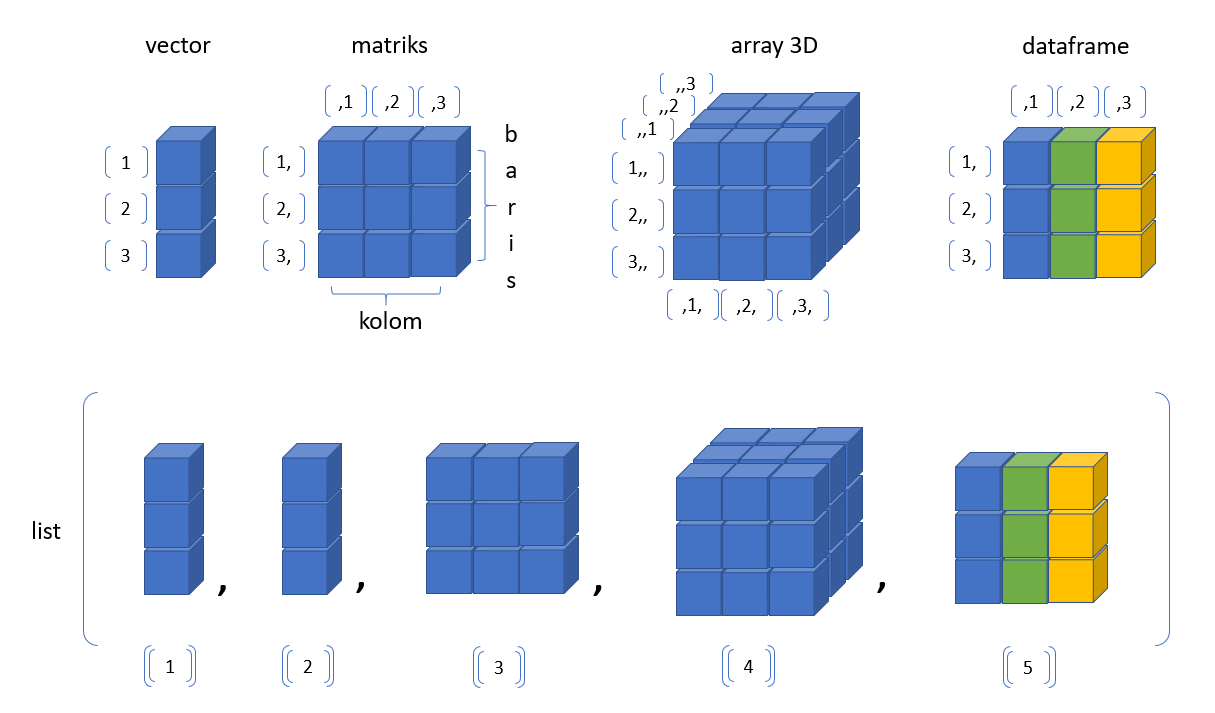
\includegraphics[width=1\linewidth]{./images/Bab3/Struktur_Data} 

}

\caption{Struktur Data dalam R}\label{fig:struktur-data}
\end{figure}

\hypertarget{vektor}{%
\section{Vektor}\label{vektor}}

Elemen paling dasar dalam R adalah vektor, yang berisikan kumpulan elemen data dengan tipe yang sama. Terdapat dua jenis vector, yaitu vector numerik dan vector karakter. Misalnya:

\begin{Shaded}
\begin{Highlighting}[]
\NormalTok{vektor }\OtherTok{\textless{}{-}} \FunctionTok{seq}\NormalTok{(}\AttributeTok{from=}\DecValTok{10}\NormalTok{, }\AttributeTok{to=}\DecValTok{21}\NormalTok{, }\AttributeTok{by=}\DecValTok{1}\NormalTok{)      }\CommentTok{\# fungsi \textasciigrave{}seq()\textasciigrave{} dengan "by"}
\NormalTok{vektor}\OtherTok{\textless{}{-}} \FunctionTok{seq}\NormalTok{(}\AttributeTok{from=}\DecValTok{10}\NormalTok{, }\AttributeTok{to=}\DecValTok{21}\NormalTok{, }\AttributeTok{len=}\DecValTok{12}\NormalTok{)     }\CommentTok{\# fungsi \textasciigrave{}seq()\textasciigrave{} dengan "len"}
\NormalTok{vektor }\OtherTok{\textless{}{-}} \DecValTok{10}\SpecialCharTok{:}\DecValTok{21}                          \CommentTok{\# tetapkan data dalam vektor }
\NormalTok{vektor }\OtherTok{\textless{}{-}}\NormalTok{ vektor}\SpecialCharTok{+}\DecValTok{2}                       \CommentTok{\# Operasi berdasarkan elemen}
\NormalTok{vektor }\OtherTok{\textless{}{-}}\NormalTok{ vektor}\SpecialCharTok{*}\DecValTok{2}                       \CommentTok{\# Tambahkan 2 untuk setiap elemen }
\NormalTok{vektor }\OtherTok{\textless{}{-}}\NormalTok{ vektor}\SpecialCharTok{\^{}}\DecValTok{2}                       \CommentTok{\# Pangkat 2 untuk setiap elemen }
\NormalTok{vektor }\OtherTok{\textless{}{-}} \FunctionTok{sqrt}\NormalTok{(vektor)                   }\CommentTok{\# Akar kuadrat untuk setiap elemen}
\NormalTok{vektor }\OtherTok{\textless{}{-}} \FunctionTok{log}\NormalTok{(vektor)                    }\CommentTok{\# Logaritma untuk setiap elemen}
\NormalTok{vektor}\OtherTok{\textless{}{-}} \FunctionTok{c}\NormalTok{(}\FloatTok{0.5}\NormalTok{, }\FloatTok{0.6}\NormalTok{)                     }\CommentTok{\# Numerik}
\NormalTok{vektor }\OtherTok{\textless{}{-}} \FunctionTok{c}\NormalTok{(}\ConstantTok{TRUE}\NormalTok{, }\ConstantTok{FALSE}\NormalTok{)                 }\CommentTok{\# Logis}
\NormalTok{vektor }\OtherTok{\textless{}{-}} \FunctionTok{c}\NormalTok{(T, F)                        }\CommentTok{\# Logis}
\NormalTok{vektor }\OtherTok{\textless{}{-}} \FunctionTok{c}\NormalTok{(}\StringTok{"a"}\NormalTok{, }\StringTok{"b"}\NormalTok{, }\StringTok{"c"}\NormalTok{)               }\CommentTok{\# Karakter}
\NormalTok{vektor }\OtherTok{\textless{}{-}} \DecValTok{9}\SpecialCharTok{:}\DecValTok{29}                           \CommentTok{\# Integer}
\NormalTok{vektor }\OtherTok{\textless{}{-}} \FunctionTok{c}\NormalTok{(}\DecValTok{1}\SpecialCharTok{+}\NormalTok{0i, }\DecValTok{2}\SpecialCharTok{+}\NormalTok{4i)                  }\CommentTok{\# Kompleks}
\NormalTok{vektor }\OtherTok{\textless{}{-}} \FunctionTok{vector}\NormalTok{(}\StringTok{"numeric"}\NormalTok{, }\AttributeTok{length =} \DecValTok{10}\NormalTok{) }\CommentTok{\# untuk inisialisasi vektor.}
\end{Highlighting}
\end{Shaded}

\textbf{Catatan:} Menurut \href{https://stat.ethz.ch/R-manual/R-devel/doc/manual/R-lang.html\#Objects}{dokumentasi R} untuk \texttt{typeof()} dan \texttt{class()}, pernyataan tentang ``perbedaan utama/main difference'' adalah tidak benar. Kelas adalah atribut dari objek yang dapat ditetapkan terlepas dari mode penyimpanan internalnya, sedangkan \texttt{typeof()} menentukan tipe (R internal) atau mode penyimpanan dari objek apa pun. Salah satu menggambarkan karakteristik logis sedangkan yang lain adalah karakteristik fisik dari suatu objek.

\begin{Shaded}
\begin{Highlighting}[]
\FunctionTok{class}\NormalTok{(vektor)                            }\CommentTok{\# Periksa kelas vektor}
\FunctionTok{as.numeric}\NormalTok{(vektor)                       }\CommentTok{\# Menetapkan vektor sebagai numerik}
\FunctionTok{as.logical}\NormalTok{(vektor)                       }\CommentTok{\# Menetapkan vektor sebagai logis}
\FunctionTok{as.character}\NormalTok{(vektor)                     }\CommentTok{\# Menetapkan vektor sebagai karakter}
\FunctionTok{as.numeric}\NormalTok{(}\FunctionTok{c}\NormalTok{(}\ConstantTok{FALSE}\NormalTok{,}\ConstantTok{TRUE}\NormalTok{,}\ConstantTok{TRUE}\NormalTok{,}\ConstantTok{FALSE}\NormalTok{))     }\CommentTok{\# Menetapkan vektor logis sebagai angka }
\end{Highlighting}
\end{Shaded}

Terkadang, R tidak dapat menemukan cara untuk memaksa suatu objek dan ini dapat menghasilkan NA.

\begin{Shaded}
\begin{Highlighting}[]
\NormalTok{vektor }\OtherTok{\textless{}{-}} \FunctionTok{c}\NormalTok{(}\StringTok{"a"}\NormalTok{, }\StringTok{"b"}\NormalTok{, }\StringTok{"c"}\NormalTok{,}\StringTok{"1"}\NormalTok{)             }\CommentTok{\# menetapkan nilai vektor}
\FunctionTok{as.numeric}\NormalTok{(vektor)                       }\CommentTok{\# menetapkan vektor sebagai numerik}
\end{Highlighting}
\end{Shaded}

\begin{verbatim}
## Warning: NAs introduced by coercion
\end{verbatim}

\begin{Shaded}
\begin{Highlighting}[]
\FunctionTok{as.logical}\NormalTok{(vektor)                       }\CommentTok{\# menetapkan vektor sebagai logis}
\FunctionTok{as.complex}\NormalTok{(vektor)                       }\CommentTok{\# menetapkan vektor sebagai karakter}
\end{Highlighting}
\end{Shaded}

\begin{verbatim}
## Warning: NAs introduced by coercion
\end{verbatim}

\textbf{Catatan:} Saat paksaan tidak masuk akal terjadi, Anda biasanya akan mendapat peringatan dari R.

Kita sudah melihat bahwa elemen dasar dari objek R adalah vektor. Vektor dapat ditetapkan dengan berbagai jenis berikut:

\begin{itemize}
\tightlist
\item
  \textbf{character:} di mana setiap elemen adalah string, mis., urutan simbol alfanumerik.
\item
  \textbf{numeric:} di mana setiap elemen adalah \href{https://en.wikipedia.org/wiki/Real_number}{bilangan real} dalam format floating point \href{https://en.wikipedia.org/wiki/Double-precision_floating-point_format}{presisi ganda}.
\item
  \textbf{integer:} di mana setiap elemen adalah \href{https://en.wikipedia.org/wiki/Integer}{integer}.
\item
  \textbf{logis:} di mana setiap elemen adalah TRUE, FALSE, atau NA3
\item
  \textbf{complex:} di mana setiap elemen adalah bilangan kompleks.
\end{itemize}

\hypertarget{matriks}{%
\section{Matriks}\label{matriks}}

Matriks adalah vektor dengan atribut dimensi. Matriks dibuat berdasarkan kolom, sehingga entri dapat dianggap dimulai dari sudut ``kiri atas'' dan mengalir di kolom.

\begin{Shaded}
\begin{Highlighting}[]
\NormalTok{matriks }\OtherTok{\textless{}{-}} \FunctionTok{matrix}\NormalTok{(}\FunctionTok{c}\NormalTok{(}\DecValTok{1}\NormalTok{, }\DecValTok{2}\NormalTok{, }\DecValTok{3}\NormalTok{, }\DecValTok{4}\NormalTok{, }\DecValTok{5}\NormalTok{, }\DecValTok{6}\NormalTok{), }\AttributeTok{nrow =} \DecValTok{2}\NormalTok{, }\AttributeTok{ncol =} \DecValTok{3}\NormalTok{)}
\NormalTok{matriks}
\end{Highlighting}
\end{Shaded}

\begin{verbatim}
##      [,1] [,2] [,3]
## [1,]    1    3    5
## [2,]    2    4    6
\end{verbatim}

Matriks juga dapat dibuat langsung dari vektor dengan menambahkan atribut dimensi.

\begin{Shaded}
\begin{Highlighting}[]
\NormalTok{matriks }\OtherTok{\textless{}{-}} \DecValTok{1}\SpecialCharTok{:}\DecValTok{6}                         \CommentTok{\# Membuat vektor}
\FunctionTok{dim}\NormalTok{(matriks) }\OtherTok{\textless{}{-}} \FunctionTok{c}\NormalTok{(}\DecValTok{2}\NormalTok{, }\DecValTok{3}\NormalTok{)                }\CommentTok{\# rubah vektor sebagai matriks sebesar 2x3}
\NormalTok{matriks                                }\CommentTok{\# Mencetak hasilnya}
\end{Highlighting}
\end{Shaded}

Matriks dapat dibuat dengan pengikatan kolom atau pengikatan baris dengan fungsi \texttt{cbind()} dan \texttt{rbind()}.

\begin{Shaded}
\begin{Highlighting}[]
\NormalTok{x }\OtherTok{\textless{}{-}} \DecValTok{1}\SpecialCharTok{:}\DecValTok{3}                              \CommentTok{\# Membuat vektor \textasciigrave{}x\textasciigrave{}}
\NormalTok{y }\OtherTok{\textless{}{-}} \DecValTok{10}\SpecialCharTok{:}\DecValTok{12}                            \CommentTok{\# Membuat vektor \textasciigrave{}y\textasciigrave{}}
\FunctionTok{cbind}\NormalTok{(x, y)                           }\CommentTok{\# Menggabungkan vektor \textasciigrave{}x\textasciigrave{} dan\textasciigrave{} y\textasciigrave{} dengan kolom}
\FunctionTok{rbind}\NormalTok{(x, y)                           }\CommentTok{\# Menggabungkan vektor \textasciigrave{}x\textasciigrave{} dan\textasciigrave{} y\textasciigrave{} dengan baris}
\end{Highlighting}
\end{Shaded}

\hypertarget{array}{%
\section{Array}\label{array}}

Array mirip dengan matrix, tetapi dapat memiliki lebih dari dua dimensi. Masing-masing dimensi dalam array memiliki ukuran tertentu.

\begin{Shaded}
\begin{Highlighting}[]
\NormalTok{array\_data }\OtherTok{\textless{}{-}} \FunctionTok{array}\NormalTok{(}\FunctionTok{c}\NormalTok{(}\DecValTok{1}\NormalTok{, }\DecValTok{2}\NormalTok{, }\DecValTok{3}\NormalTok{, }\DecValTok{4}\NormalTok{, }\DecValTok{5}\NormalTok{, }\DecValTok{6}\NormalTok{), }\AttributeTok{dim =} \FunctionTok{c}\NormalTok{(}\DecValTok{2}\NormalTok{, }\DecValTok{3}\NormalTok{, }\DecValTok{1}\NormalTok{))}
\end{Highlighting}
\end{Shaded}

\hypertarget{faktor}{%
\section{Faktor}\label{faktor}}

Faktor-faktor digunakan untuk mewakili data kategorikal dan dapat menjadi tidak teratur atau teratur. Orang dapat menganggap faktor sebagai vektor integer di mana setiap integer memiliki label. Menggunakan faktor dengan label lebih baik daripada menggunakan bilangan bulat karena faktor menggambarkan diri sendiri. Memiliki variabel yang memiliki nilai ``Laki-laki'' dan ``Perempuan'' lebih baik daripada variabel yang memiliki nilai 1 dan 2. Objek-objek dapat dibuat dengan fungsi \texttt{faktor()}.

\begin{Shaded}
\begin{Highlighting}[]
\NormalTok{x }\OtherTok{\textless{}{-}} \FunctionTok{factor}\NormalTok{(}\FunctionTok{c}\NormalTok{(}\StringTok{"yes"}\NormalTok{,}\StringTok{"no"}\NormalTok{,}\StringTok{"yes"}\NormalTok{,}\StringTok{"no"}\NormalTok{))  }\CommentTok{\# Membuat objek faktor}
\NormalTok{x                                      }\CommentTok{\# Cetak hasilnya}
\FunctionTok{table}\NormalTok{(x)                               }\CommentTok{\# Tabel dari \textasciigrave{}x\textasciigrave{}}
\FunctionTok{unclass}\NormalTok{(x)                             }\CommentTok{\# Melihat representasi faktor yang mendasarinya}
\FunctionTok{attr}\NormalTok{(x,}\StringTok{"levels"}\NormalTok{)                       }\CommentTok{\# Melihat representasi faktor yang mendasarinya}
\end{Highlighting}
\end{Shaded}

\hypertarget{data-frame}{%
\section{Data Frame}\label{data-frame}}

Kerangka data (data frame) adalah tabel atau struktur mirip array dua dimensi di mana setiap kolom berisi nilai satu variabel dan setiap baris berisi satu set nilai dari setiap kolom.

Berikut ini adalah karakteristik data frame.

\begin{itemize}
\tightlist
\item
  Nama kolom tidak boleh kosong;
\item
  Nama baris harus unik;
\item
  Data yang disimpan dalam data frame bisa dari numerik, faktor atau tipe karakter;
\item
  Setiap kolom harus berisi jumlah item data yang sama.
\end{itemize}

\begin{Shaded}
\begin{Highlighting}[]
\CommentTok{\# Buat data frame pertama.}
\NormalTok{df1 }\OtherTok{\textless{}{-}} \FunctionTok{data.frame}\NormalTok{(}\AttributeTok{id =} \FunctionTok{c}\NormalTok{ (}\DecValTok{1}\SpecialCharTok{:}\DecValTok{5}\NormalTok{), }
                \AttributeTok{name =} \FunctionTok{c}\NormalTok{(}\StringTok{"Julian"}\NormalTok{,}\StringTok{"Vanessa"}\NormalTok{,}\StringTok{"Jeffry"}\NormalTok{,}\StringTok{"Angel"}\NormalTok{,}\StringTok{"Nikki"}\NormalTok{),}
              \AttributeTok{salary =} \FunctionTok{c}\NormalTok{(}\FloatTok{623.3}\NormalTok{,}\FloatTok{515.2}\NormalTok{,}\FloatTok{611.0}\NormalTok{,}\FloatTok{729.0}\NormalTok{,}\FloatTok{843.25}\NormalTok{), }
          \AttributeTok{start\_date =} \FunctionTok{as.Date}\NormalTok{(}\FunctionTok{c}\NormalTok{(}\StringTok{"2022{-}01{-}01"}\NormalTok{, }\StringTok{"2022{-}09{-}23"}\NormalTok{, }\StringTok{"2022{-}11{-}15"}\NormalTok{,                                               }\StringTok{"2022{-}05{-}11"}\NormalTok{, }\StringTok{"2022{-}03{-}27"}\NormalTok{)),}
                \AttributeTok{dept =} \FunctionTok{c}\NormalTok{(}\StringTok{"DS"}\NormalTok{,}\StringTok{"DS"}\NormalTok{,}\StringTok{"BA"}\NormalTok{,}\StringTok{"DA"}\NormalTok{,}\StringTok{"DS"}\NormalTok{), }\AttributeTok{stringsAsFactors =}\NormalTok{ F)}
\NormalTok{df1}
\end{Highlighting}
\end{Shaded}

\begin{Shaded}
\begin{Highlighting}[]
\CommentTok{\# Buat data frame kedua.}
\NormalTok{df2 }\OtherTok{\textless{}{-}}\FunctionTok{data.frame}\NormalTok{(}\AttributeTok{id =} \FunctionTok{c}\NormalTok{ (}\DecValTok{6}\SpecialCharTok{:}\DecValTok{10}\NormalTok{), }
               \AttributeTok{name =} \FunctionTok{c}\NormalTok{(}\StringTok{"Ardifo"}\NormalTok{,}\StringTok{"Irene"}\NormalTok{,}\StringTok{"Kefas"}\NormalTok{,}\StringTok{"Sherly"}\NormalTok{,}\StringTok{"Bakti"}\NormalTok{),}
             \AttributeTok{salary =} \FunctionTok{c}\NormalTok{(}\FloatTok{578.0}\NormalTok{,}\FloatTok{722.5}\NormalTok{,}\FloatTok{632.8}\NormalTok{,}\FloatTok{632.8}\NormalTok{,}\ConstantTok{NA}\NormalTok{), }
         \AttributeTok{start\_date =} \FunctionTok{as.Date}\NormalTok{(}\FunctionTok{c}\NormalTok{(}\StringTok{"2022{-}05{-}21"}\NormalTok{,}\StringTok{"2022{-}07{-}30"}\NormalTok{,}\StringTok{"2022{-}06{-}17"}\NormalTok{,}
                                \StringTok{"2022{-}07{-}30"}\NormalTok{,}\StringTok{"2018{-}09{-}03"}\NormalTok{)),}
               \AttributeTok{dept =} \FunctionTok{c}\NormalTok{(}\StringTok{"Actuaries"}\NormalTok{,}\StringTok{"Actuaries"}\NormalTok{,}\StringTok{"CA"}\NormalTok{,}\StringTok{"DE"}\NormalTok{,}\StringTok{"Lecturer"}\NormalTok{),}\AttributeTok{stringsAsFactors =}\NormalTok{ F)}
\NormalTok{df2}
\end{Highlighting}
\end{Shaded}

\begin{Shaded}
\begin{Highlighting}[]
\NormalTok{df3 }\OtherTok{\textless{}{-}} \FunctionTok{rbind}\NormalTok{(df1,df2)                  }\CommentTok{\# Gabungkan dua frame data}
\FunctionTok{print}\NormalTok{(df3)                             }\CommentTok{\# Cetak hasilnya \textasciigrave{}df3\textasciigrave{}}
\FunctionTok{head}\NormalTok{(df3)                              }\CommentTok{\# Cetak enam baris pertama}
\FunctionTok{head}\NormalTok{(df3,}\DecValTok{6}\NormalTok{)                            }\CommentTok{\# Cetak enam baris pertama}
\CommentTok{\#View(df3)                             \# Menggunakan RStudio seperti penampil Excel}
\FunctionTok{class}\NormalTok{(df3)                             }\CommentTok{\# objeknya bertipe data.frame}
\FunctionTok{str}\NormalTok{(df3)                               }\CommentTok{\# Dapatkan struktur data frame}
\FunctionTok{dim}\NormalTok{(df3)                               }\CommentTok{\# Periksa dimensi data}
\end{Highlighting}
\end{Shaded}

Data frame biasanya dibuat dengan membaca dalam dataset menggunakan \texttt{read.table()} atau \texttt{read.csv\ ()}. Namun, data frame juga dapat dibuat secara eksplisit dengan fungsi \texttt{data.frame()} atau mereka dapat dipaksakan dari jenis objek lain seperti list.

\hypertarget{lists}{%
\section{Lists}\label{lists}}

List dalam R adalah struktur data yang mengizinkan Anda untuk menyimpan berbagai jenis objek, termasuk vektor, matriks, array, dataframe, dan objek list lainnya, dalam satu objek tunggal. Ini memungkinkan Anda untuk membuat struktur data yang kompleks dan fleksibel dengan menggabungkan objek-objek yang berbeda ke dalam satu wadah. List sering digunakan ketika Anda perlu mengorganisir dan mengelompokkan objek-objek yang terkait.

Berikut adalah contoh penggunaan dan pembuatan list dalam R:

\begin{Shaded}
\begin{Highlighting}[]
\CommentTok{\# Membuat vektor dan matriks}
\NormalTok{vektor }\OtherTok{\textless{}{-}} \FunctionTok{c}\NormalTok{(}\FloatTok{1.5}\NormalTok{, }\FloatTok{2.7}\NormalTok{, }\FloatTok{3.2}\NormalTok{, }\FloatTok{4.0}\NormalTok{)}
\NormalTok{matriks }\OtherTok{\textless{}{-}} \FunctionTok{matrix}\NormalTok{(}\FunctionTok{c}\NormalTok{(}\DecValTok{1}\NormalTok{, }\DecValTok{2}\NormalTok{, }\DecValTok{3}\NormalTok{, }\DecValTok{4}\NormalTok{, }\DecValTok{5}\NormalTok{, }\DecValTok{6}\NormalTok{), }\AttributeTok{nrow =} \DecValTok{2}\NormalTok{, }\AttributeTok{ncol =} \DecValTok{3}\NormalTok{)}
\end{Highlighting}
\end{Shaded}

\begin{Shaded}
\begin{Highlighting}[]
\CommentTok{\# Membuat dataframe}
\NormalTok{data\_frame }\OtherTok{\textless{}{-}} \FunctionTok{data.frame}\NormalTok{(}\AttributeTok{name =} \FunctionTok{c}\NormalTok{(}\StringTok{"Alice"}\NormalTok{, }\StringTok{"Bakti"}\NormalTok{, }\StringTok{"Charlie"}\NormalTok{),}
                         \AttributeTok{age =} \FunctionTok{c}\NormalTok{(}\DecValTok{25}\NormalTok{, }\DecValTok{30}\NormalTok{, }\DecValTok{28}\NormalTok{),}
                         \AttributeTok{score =} \FunctionTok{c}\NormalTok{(}\DecValTok{95}\NormalTok{, }\DecValTok{88}\NormalTok{, }\DecValTok{76}\NormalTok{))}
\end{Highlighting}
\end{Shaded}

\begin{Shaded}
\begin{Highlighting}[]
\NormalTok{faktor }\OtherTok{\textless{}{-}} \StringTok{"List, Sudah Jadi"}
\end{Highlighting}
\end{Shaded}

\begin{Shaded}
\begin{Highlighting}[]
\CommentTok{\# Membuat list}
\NormalTok{my\_list }\OtherTok{\textless{}{-}} \FunctionTok{list}\NormalTok{(vektor, matriks, data\_frame, faktor)}
\end{Highlighting}
\end{Shaded}

\begin{Shaded}
\begin{Highlighting}[]
\CommentTok{\# Menampilkan list}
\FunctionTok{print}\NormalTok{(my\_list)}
\end{Highlighting}
\end{Shaded}

Anda juga dapat memberi nama pada setiap elemen dalam list untuk membuat list yang lebih mudah dibaca:

\begin{Shaded}
\begin{Highlighting}[]
\NormalTok{nama\_list }\OtherTok{\textless{}{-}} \FunctionTok{list}\NormalTok{(}\AttributeTok{elemen1 =}\NormalTok{ vektor, }
                  \AttributeTok{elemen2 =}\NormalTok{ matriks, }
                  \AttributeTok{elemen3 =}\NormalTok{ data\_frame, }
                  \AttributeTok{elemen4 =}\NormalTok{ faktor)}

\CommentTok{\# Menampilkan elemen dalam list berdasarkan nama}
\FunctionTok{print}\NormalTok{(nama\_list}\SpecialCharTok{$}\NormalTok{elemen1)}
\end{Highlighting}
\end{Shaded}

\begin{verbatim}
## [1] 1.5 2.7 3.2 4.0
\end{verbatim}

\begin{Shaded}
\begin{Highlighting}[]
\FunctionTok{print}\NormalTok{(nama\_list}\SpecialCharTok{$}\NormalTok{elemen2)}
\end{Highlighting}
\end{Shaded}

\begin{verbatim}
##      [,1] [,2] [,3]
## [1,]    1    3    5
## [2,]    2    4    6
\end{verbatim}

\begin{Shaded}
\begin{Highlighting}[]
\FunctionTok{print}\NormalTok{(nama\_list}\SpecialCharTok{$}\NormalTok{elemen3)}
\end{Highlighting}
\end{Shaded}

\begin{verbatim}
##      name age score
## 1   Alice  25    95
## 2   Bakti  30    88
## 3 Charlie  28    76
\end{verbatim}

\begin{Shaded}
\begin{Highlighting}[]
\FunctionTok{print}\NormalTok{(nama\_list}\SpecialCharTok{$}\NormalTok{elemen4)}
\end{Highlighting}
\end{Shaded}

\begin{verbatim}
## [1] "List, Sudah Jadi"
\end{verbatim}

Anda dapat mengakses elemen-elemen dalam list menggunakan indeks atau nama. Misalnya:

\begin{Shaded}
\begin{Highlighting}[]
\CommentTok{\# Mengakses elemen pertama dalam list menggunakan indeks}
\NormalTok{elemen1 }\OtherTok{\textless{}{-}}\NormalTok{ my\_list[[}\DecValTok{1}\NormalTok{]]}
\NormalTok{elemen2 }\OtherTok{\textless{}{-}}\NormalTok{ my\_list[[}\DecValTok{2}\NormalTok{]]}
\NormalTok{elemen3 }\OtherTok{\textless{}{-}}\NormalTok{ my\_list[[}\DecValTok{2}\NormalTok{]]}
\NormalTok{elemen4 }\OtherTok{\textless{}{-}}\NormalTok{ my\_list[[}\DecValTok{2}\NormalTok{]]}

\CommentTok{\# Menampilkan hasil}
\FunctionTok{print}\NormalTok{(elemen1)}
\FunctionTok{print}\NormalTok{(elemen2)}
\FunctionTok{print}\NormalTok{(elemen3)}
\FunctionTok{print}\NormalTok{(elemen4)}
\end{Highlighting}
\end{Shaded}

List memungkinkan Anda mengorganisir, mengelompokkan, dan mengakses objek-objek yang beragam dalam struktur data tunggal, sehingga sangat berguna dalam analisis data yang kompleks dan beragam.

\hypertarget{rekayasa-data-frame}{%
\section{Rekayasa Data Frame}\label{rekayasa-data-frame}}

\hypertarget{tanpa-packages}{%
\subsection{Tanpa Packages}\label{tanpa-packages}}

Sebagai seorang Data Scientist, ketika mencoba menyimulasikan proses analisis data, pemodelan, bahkan prediksi. Anda harus mampu secara intuitif membangun dataframe untuk memperkirakan kumpulan data sampel. Terutama, ketika Anda tidak memiliki kumpulan data sampel sama sekali. Oleh karena itu, pada bagian ini, kita akan belajar sedikit mengenai cara menghasilkan dataframe. Harap perhatikan baik-baik contoh berikut:

\begin{Shaded}
\begin{Highlighting}[]
\CommentTok{\# Misalkan Anda ingin membangun kumpulan data karyawan di sebuah perusahaan}

\NormalTok{No}\OtherTok{\textless{}{-}}\NormalTok{(}\DecValTok{1}\SpecialCharTok{:}\DecValTok{52}\NormalTok{)                                       }\CommentTok{\# Menghasilkan bilangan 1{-}52}
\NormalTok{Name}\OtherTok{\textless{}{-}}\FunctionTok{c}\NormalTok{(LETTERS,letters)                         }\CommentTok{\# 26 LETTERS dan 26 letters}
\NormalTok{Gender}\OtherTok{\textless{}{-}}\FunctionTok{sample}\NormalTok{(}\FunctionTok{rep}\NormalTok{(}\FunctionTok{c}\NormalTok{(}\StringTok{"Male"}\NormalTok{,}\StringTok{"Female"}\NormalTok{),}\AttributeTok{times=}\DecValTok{26}\NormalTok{)) }\CommentTok{\# 26 Laki{-}laki dan 26 perempuan}

\CommentTok{\# Menghasilkan tanggal lahir}
\NormalTok{year\_in\_3}\OtherTok{\textless{}{-}}\FunctionTok{seq}\NormalTok{(}\FunctionTok{as.Date}\NormalTok{(}\StringTok{"2000/01/01"}\NormalTok{), }\AttributeTok{by=}\StringTok{"year"}\NormalTok{, }\AttributeTok{length.out=}\DecValTok{4}\NormalTok{)}
\NormalTok{Birthday }\OtherTok{\textless{}{-}} \FunctionTok{rep}\NormalTok{(year\_in\_3, }\AttributeTok{times=}\DecValTok{13}\NormalTok{)}

\CommentTok{\# Menghasilkan kategori universitas}
\NormalTok{univ1}\OtherTok{\textless{}{-}}\FunctionTok{rep}\NormalTok{(}\StringTok{"National"}\NormalTok{,}\AttributeTok{times=}\DecValTok{26}\NormalTok{)                  }\CommentTok{\# 26 universitas negeri}
\NormalTok{univ2}\OtherTok{\textless{}{-}}\FunctionTok{rep}\NormalTok{(}\StringTok{"Private"}\NormalTok{,}\AttributeTok{times=}\DecValTok{16}\NormalTok{)                   }\CommentTok{\# 16 universitas swasta }
\NormalTok{univ3}\OtherTok{\textless{}{-}}\FunctionTok{rep}\NormalTok{(}\StringTok{"Overseas"}\NormalTok{,}\AttributeTok{times=}\DecValTok{10}\NormalTok{)                  }\CommentTok{\# 10 universitas luar negeri}
\NormalTok{Universities}\OtherTok{\textless{}{-}}\FunctionTok{sample}\NormalTok{(}\FunctionTok{c}\NormalTok{(univ1,univ2,univ3))       }\CommentTok{\# Menggabungkan data (vetor)}

\NormalTok{gpa}\OtherTok{\textless{}{-}}\FunctionTok{runif}\NormalTok{(}\DecValTok{52}\NormalTok{,}\AttributeTok{min=}\FloatTok{3.00}\NormalTok{,}\AttributeTok{max=}\FloatTok{4.00}\NormalTok{)                 }\CommentTok{\# Menghasilkan 52 bilangan acak (min=3, dan max=4) }
\NormalTok{GPA}\OtherTok{\textless{}{-}}\FunctionTok{round}\NormalTok{(gpa,}\AttributeTok{digits=}\DecValTok{2}\NormalTok{)                         }\CommentTok{\# Mengatur digit bilangan acak Anda}
\NormalTok{Salary}\OtherTok{\textless{}{-}}\FunctionTok{sample}\NormalTok{(}\DecValTok{600}\SpecialCharTok{:}\DecValTok{1200}\NormalTok{,}\DecValTok{52}\NormalTok{,}\AttributeTok{replace=}\NormalTok{T)            }\CommentTok{\# Menghasilakn sampel antara 600{-}1200 (memungkinkan nilai duplikat)}
\NormalTok{Employees}\OtherTok{\textless{}{-}}\FunctionTok{data.frame}\NormalTok{(No,}
\NormalTok{                      Name,}
\NormalTok{                      Birthday,}
\NormalTok{                      Gender,}
\NormalTok{                      Universities,}
\NormalTok{                      GPA,}
\NormalTok{                      Salary)}
\NormalTok{Employees}
\end{Highlighting}
\end{Shaded}

\begin{verbatim}
##    No Name   Birthday Gender Universities  GPA Salary
## 1   1    A 2000-01-01 Female      Private 3.97   1012
## 2   2    B 2001-01-01   Male      Private 3.07   1016
## 3   3    C 2002-01-01 Female     Overseas 3.69    985
## 4   4    D 2003-01-01   Male      Private 3.28    981
## 5   5    E 2000-01-01   Male      Private 3.53    720
## 6   6    F 2001-01-01 Female     National 3.30   1122
## 7   7    G 2002-01-01   Male      Private 3.58    754
## 8   8    H 2003-01-01   Male      Private 3.38    999
## 9   9    I 2000-01-01 Female     National 3.47   1200
## 10 10    J 2001-01-01 Female     National 3.78    886
## 11 11    K 2002-01-01 Female     Overseas 3.25    891
## 12 12    L 2003-01-01   Male     Overseas 3.53    809
## 13 13    M 2000-01-01   Male     National 3.72    605
## 14 14    N 2001-01-01 Female     National 3.92    977
## 15 15    O 2002-01-01 Female     Overseas 3.83    822
## 16 16    P 2003-01-01 Female     Overseas 3.59    930
## 17 17    Q 2000-01-01   Male     National 3.08    672
## 18 18    R 2001-01-01 Female      Private 3.22   1139
## 19 19    S 2002-01-01   Male     National 3.11    990
## 20 20    T 2003-01-01   Male      Private 3.76    913
## 21 21    U 2000-01-01 Female     National 3.45    754
## 22 22    V 2001-01-01   Male     National 3.86   1166
## 23 23    W 2002-01-01   Male      Private 3.58   1128
## 24 24    X 2003-01-01 Female     National 3.92    971
## 25 25    Y 2000-01-01   Male     Overseas 3.66    841
## 26 26    Z 2001-01-01   Male      Private 3.86    825
## 27 27    a 2002-01-01   Male     National 3.30    815
## 28 28    b 2003-01-01 Female     National 3.08    956
## 29 29    c 2000-01-01   Male     National 3.16    815
## 30 30    d 2001-01-01   Male     National 3.02    773
## 31 31    e 2002-01-01 Female     National 3.07   1022
## 32 32    f 2003-01-01 Female      Private 3.57    708
## 33 33    g 2000-01-01 Female     National 3.42    971
## 34 34    h 2001-01-01   Male     National 3.23    992
## 35 35    i 2002-01-01 Female      Private 3.22   1014
## 36 36    j 2003-01-01 Female      Private 3.24    775
## 37 37    k 2000-01-01 Female     National 3.43   1071
## 38 38    l 2001-01-01   Male      Private 3.29   1062
## 39 39    m 2002-01-01   Male      Private 3.59    799
## 40 40    n 2003-01-01   Male     Overseas 3.86    989
## 41 41    o 2000-01-01   Male     National 3.44    730
## 42 42    p 2001-01-01 Female     National 3.92    972
## 43 43    q 2002-01-01 Female     National 3.59    668
## 44 44    r 2003-01-01   Male     National 3.32   1073
## 45 45    s 2000-01-01 Female      Private 3.18   1061
## 46 46    t 2001-01-01   Male     National 3.67    754
## 47 47    u 2002-01-01 Female     National 3.42   1066
## 48 48    v 2003-01-01 Female     Overseas 3.10    855
## 49 49    w 2000-01-01 Female     Overseas 3.40   1098
## 50 50    x 2001-01-01 Female     National 3.26    693
## 51 51    y 2002-01-01   Male     National 3.28    607
## 52 52    z 2003-01-01   Male     Overseas 3.10    634
\end{verbatim}

\hypertarget{mengunakan-packages}{%
\subsection{Mengunakan Packages}\label{mengunakan-packages}}

Dalam contoh kedua ini, digunakan pustaka \emph{(Packages)} \texttt{faker} untuk menghasilkan data palsu seperti nama, alamat, dan lain-lain. Pastikan Anda telah menginstal pustaka tersebut menggunakan perintah \texttt{install.packages("fakir")} jika belum terinstal, mengikuti langkah berikut.

\begin{Shaded}
\begin{Highlighting}[]
\FunctionTok{install.packages}\NormalTok{(}\StringTok{"remotes"}\NormalTok{)}
\NormalTok{remotes}\SpecialCharTok{::}\FunctionTok{install\_github}\NormalTok{(}\StringTok{"ThinkR{-}open/fakir"}\NormalTok{)}
\end{Highlighting}
\end{Shaded}

Selanjutnya, anda dapat membuat data frame palsu seperti diperlihatkan berikut:

\begin{Shaded}
\begin{Highlighting}[]
\FunctionTok{library}\NormalTok{(fakir)}
\FunctionTok{fake\_ticket\_client}\NormalTok{(}\AttributeTok{vol =} \DecValTok{10}\NormalTok{)}
\end{Highlighting}
\end{Shaded}

\begin{verbatim}
## # A tibble: 10 x 25
##    ref        num_client first last  job     age region
##    <chr>      <chr>      <chr> <chr> <chr> <dbl> <chr> 
##  1 DOSS-AMQN~ 79         Jovan O'Ke~ Gene~    22 Prove~
##  2 DOSS-NCKJ~ 69         Miss  Lean~ Emer~    68 Haute~
##  3 DOSS-GPBE~ 120        Odell Stok~ Engi~    24 Auver~
##  4 DOSS-GRLN~ 31         Loren Lars~ <NA>     NA Midi-~
##  5 DOSS-LEPJ~ 59         Mayb~ Maye~ Furt~    18 Aquit~
##  6 DOSS-DUCL~ 118        Jama~ Ober~ Engi~    18 Île-d~
##  7 DOSS-OCED~ 77         Lee   Scha~ Admi~    NA Poito~
##  8 DOSS-KXSJ~ 65         Deme~ Auer  Cont~    21 Midi-~
##  9 DOSS-UITD~ 141        Wilf~ Harv~ Educ~    53 <NA>  
## 10 DOSS-SHKL~ 182        Addy~ Nien~ Earl~    65 Rhône~
## # i 18 more variables: id_dpt <chr>,
## #   departement <chr>, cb_provider <chr>, name <chr>,
## #   entry_date <dttm>, fidelity_points <dbl>,
## #   priority_encoded <dbl>, priority <fct>,
## #   timestamp <date>, year <dbl>, month <dbl>,
## #   day <int>, supported <chr>,
## #   supported_encoded <int>, type <chr>, ...
\end{verbatim}

\textbf{Catatan:} Pustaka \texttt{fakir} Menyimpan beberapa dataset didalamnya, antara lain:

\begin{Shaded}
\begin{Highlighting}[]
\FunctionTok{fake\_products}\NormalTok{(}\DecValTok{10}\NormalTok{)                                   }\CommentTok{\# Rekayasa Data Produk }
\FunctionTok{fake\_visits}\NormalTok{(}\AttributeTok{from =} \StringTok{"2017{-}01{-}01"}\NormalTok{, }\AttributeTok{to =} \StringTok{"2017{-}01{-}31"}\NormalTok{) }\CommentTok{\# Pengunjung Website}
\FunctionTok{fake\_sondage\_answers}\NormalTok{(}\AttributeTok{n =} \DecValTok{10}\NormalTok{)                        }\CommentTok{\# Kuisioner transfortasi}
\end{Highlighting}
\end{Shaded}

\hypertarget{latihan-1}{%
\section{Latihan}\label{latihan-1}}

\begin{enumerate}
\def\labelenumi{\arabic{enumi}.}
\item
  Buatlah Rekayasa dataframe Mahasiswa dengan empat kolom: ``Nama'', ``Usia'', ``Kota'', dan ``Nilai''. Sebanyak 100 baris, dengan syarat tidak boleh ada nama yang sama.
\item
  Buatlah Rekayasa dataframe Karyawan dengan tujuh kolom: ``No'', ``Name'', ``Birthday'', ``Gender'', ``Universities'', ``GPA'', ``Salary''. Sebanyak 100 baris, dengan syarat tidak boleh ada nama yang sama.
\item
  Buatlah Rekayasa dataframe pengunjung Website, sebanyak 200 baris.
\end{enumerate}

\textbf{Catatan:} Kumpulkan hasil latihan anda, tidak boleh sama dengan teman mahasiwa lainnya.

\hypertarget{referensi}{%
\chapter{Referensi}\label{referensi}}

Berikut adalah beberapa referensi yang dapat Anda gunakan untuk mempelajari dasar-dasar pemrograman dalam bahasa R:

\begin{enumerate}
\def\labelenumi{\arabic{enumi}.}
\tightlist
\item
  Venables, W.N. Smith D.M. and R Core Team. 2018. \textbf{An Introduction to R}: \url{https://cran.r-project.org/manuals.html}
\item
  R for Data Science: \url{https://r4ds.had.co.nz/}
\item
  Codecademy - Learn R : \url{https://www.codecademy.com/learn/learn-r}
\item
  DataCamp: \url{https://www.datacamp.com/courses/tech:r}
\item
  Primartha, R. 2018. \textbf{Belajar Machine Learning Teori dan Praktik}. Penerbit Informatika : Bandung
\item
  Rosadi,D. 2016. \textbf{Analisis Statistika dengan R}. Gadjah Mada University Press: Yogyakarta
\item
  STHDA. Running RStudio and Setting Up Your Working Directory - Easy R Programming .\url{http://www.sthda.com/english/wiki/running-rstudio-and-setting-up-your-working-directory-easy-r-programming\#set-your-working-directory}
\item
  STDHA. \textbf{Getting Help With Functions In R Programming}. \url{http://www.sthda.com/english/wiki/getting-help-with-functions-in-r-programming} .
\end{enumerate}

  \bibliography{book.bib,packages.bib}

\end{document}
